\documentclass{article}
\usepackage[utf8]{inputenc}

\title{RM Econometrics and Statistics}
\author{Clara Brünn, Christopher Thiemann and David Poth }
\date{October 2018}

\usepackage{natbib}
\usepackage{listings}
\usepackage{graphicx}
\usepackage{amssymb,amsfonts,amsthm,mathtools}
\usepackage{tikz}
\usepackage{url} % needed for waf
\usepackage{todonotes}
%\usepackage{bbm}
\usepackage{booktabs}
\usepackage{placeins}
\usepackage{subcaption}
%\usepackage{singlespacing}{setspace}
%\usepackage[colorlinks,
%pdfpagelabels,
%pdfstartview = FitH,
%bookmarksopen = true,
%bookmarksnumbered = true,
%linkcolor = black,
%plainpages = false,
%hypertexnames = false,
%citecolor = black] {hyperref}    %This package enables links to sections from table of contents etc.
\theoremstyle{definition}
\newtheorem{theorem}{Theorem}
\newtheorem{definition}[theorem]{Definition}
\newtheorem{lemma}[theorem]{Lemma}
\DeclareMathOperator*{\argmin}{arg\,min}
\DeclareMathOperator*{\sgn}{sgn}
\bibliographystyle{alpha}
\usepackage[pdf]{graphviz}


\mathchardef\ordinarycolon\mathcode`\:
\mathcode`\:=\string"8000
\begingroup \catcode`\:=\active
\gdef:{\mathrel{\mathop\ordinarycolon}}
\endgroup

% python
% Default fixed font does not support bold face
\DeclareFixedFont{\ttb}{T1}{txtt}{bx}{n}{8} % for bold
\DeclareFixedFont{\ttm}{T1}{txtt}{m}{n}{8}  % for normal

\usepackage{color}
\definecolor{deepblue}{rgb}{0,0,0.5}
\definecolor{deepred}{rgb}{0.6,0,0}
\definecolor{deepgreen}{rgb}{0,0.5,0}
\usepackage{listings}

\newcommand\pythonstyle{\lstset{
language=Python,
basicstyle=\ttm,
otherkeywords={self},             % Add keywords here
keywordstyle=\ttb\color{deepblue},
emph={MyClass,__init__},          % Custom highlighting
emphstyle=\ttb\color{deepred},    % Custom highlighting style
stringstyle=\color{deepgreen},
frame=tb,                         % Any extra options here
showstringspaces=false            % 
}}

% Python environment
\lstnewenvironment{python}[1][]
{
\pythonstyle
\lstset{#1}
}
{}

% Python for external files
\newcommand\pythonexternal[2][]{{
\pythonstyle
\lstinputlisting[#1]{#2}}}

% Python for inline
\newcommand\pythoninline[1]{{\pythonstyle\lstinline!#1!}}


\begin{document}


\begin{titlepage} % Suppresses displaying the page number on the title page and the subsequent page counts as page 1
	\newcommand{\HRule}{\rule{\linewidth}{0.5mm}} % Defines a new command for horizontal lines, change thickness here
	
	\center % Centre everything on the page
	
	%------------------------------------------------
	%  Headings
	%------------------------------------------------
	
	\textsc{\LARGE University of Bonn}\\[1.5cm] % Main heading such as the name of your university/college
	
	\textsc{\Large Research Module Econometrics and Statistics}\\[0.5cm] % Major heading such as course name
	
	\textsc{\large Term paper}\\[0.5cm] % Minor heading such as course title
	
	%------------------------------------------------
	%	Title
	%------------------------------------------------
	
	\HRule\\[0.4cm]
	
	{\huge\bfseries Fused Lasso}\\[0.4cm] % Title of your document
	
	\HRule\\[1.5cm]
	
	%------------------------------------------------
	%	Author(s)
	%------------------------------------------------
	
	\begin{minipage}{0.4\textwidth}
		\begin{flushleft}
			\large
			\textit{Author's}\\
			Clara  	\textsc{Brünn} \newline
			David   \textsc{Poth} \newline
			Christopher	\textsc{Thiemann genannt Trappmann}% Your name
		\end{flushleft}
	\end{minipage}
	~
	\begin{minipage}{0.4\textwidth}
		\begin{flushright}
			\large
			\textit{Supervisor}\\
			Prof. Dr. Dominik \textsc{Liebl} % Supervisor's name
		\end{flushright}
	\end{minipage}
	
	% If you don't want a supervisor, uncomment the two lines below and comment the code above
	%{\large\textit{Author}}\\
	%John \textsc{Smith} % Your name
	
	%------------------------------------------------
	%	Date
	%------------------------------------------------
	
	\vfill\vfill\vfill % Position the date 3/4 down the remaining page
	
	{\large\today} % Date, change the \today to a set date if you want to be precise
	
	%------------------------------------------------
	%	Logo
	%------------------------------------------------
	
	%\vfill\vfill
	%\includegraphics[width=0.2\textwidth]{placeholder.jpg}\\[1cm] % Include a department/university logo - this will require the graphicx package
	 
	%----------------------------------------------------------------------------------------
	
	\vfill % Push the date up 1/4 of the remaining page
	
\end{titlepage} \newpage

\pagenumbering{Roman}

\tableofcontents \newpage

\addcontentsline{toc}{section}{List of Figures}

\listoffigures

\addcontentsline{toc}{section}{List of Tables}

\listoftables 
\newpage 

\pagenumbering{arabic}
\addtocontents{toc}{\protect\setcounter{tocdepth}{2}}
\section{Introduction}




Methods for dealing with high-dimensional data are increasingly relevant in nearly all sciences among these empirical economics. This is due to the often high-dimensional nature of data nowadays. In particular data where the number of regressors $p$ by far exceeds the number of observations $N$.

When analyzing high-dimensional data traditional methods as ordinary least squares turn out not to be appropriate. With traditional methods one is likely to encounter infeasible computation times, non-unique solutions and overfitting. Without constraints the OLS estimator would for example fit the data perfectly for $p$ equal to $N$, resulting in weak out-of-sample forecasts. The reason is that the fit captures the noise of the given sample and not only the true underlying model of regressors and outcome. In such a case we say the model is overfit.
In order to analyze high-dimensional data “regularization” becomes necessary. This means the estimators need to be constrained in their degrees of freedom in order to avoid overfitting \citep{belloni2014}.
%complexity regularization will be necessary.  We focus here on regularizationwith the l1-penalty.

We examine one of the established methods for dealing with this kind of set-up, the Least Absolute Shrinkage and Selection Operator, short lasso and a modification of it, the fused lasso. Both are outputs of a penalized least squares regression.

% Historical context
The Lasso was introduced by \citet{lasso}. Thereafter a lot of extensions were and still are being proposed. The most prominent are the elastic net by \citet{zou2005regularization}, the fused lasso by \citet{fused}, the adaptive lasso by \citet{zou2006adaptive} and  the group lasso by \citet{meier2008group}. The idea of a fusion penalty goes back to \citet{land1996variable}, they did not combine the fusion penalty with an $\ell_1$-penalty though.
Recent literature even combines the extensions for example  \citet{bleakley2011group} present the grouped fused lasso.

The aim of this paper is to give a brief overview of lasso and fused lasso, to analyze their properties in a simulation study and to apply fused lasso on a real data application. 

%Structure
The paper is organized as follows. In section 2 we introduce lasso, define its optimization problem and investigate some interesting properties. In section 3 we present the fused lasso as an extension of the lasso, describe its behavior and properties. We provide some insights on the solution method. This is followed by a sketch of the fused lasso signal approximator, which is later used for our real data application. Asymptotic results for both lasso and fused lasso are outlined in section 4. We propose a python implementation of the fused lasso estimator in section 5. In section 6 we present a simulation study comparing the performance of the fused lasso with the lasso and another penalized regression. An application of the fused lasso to genomic data is discussed in section 7.
%We start by introducing the lasso. We define the optimization problem and give some properties thereof. After that we take a closer look at the estimator itself and show some basic properties and give intuitive explanations for the more advanced properties. We will also state some asymptotic results. The end of this chapter will give an idea on how to compute the estimator. The next chapter will then focus on the fused lasso which will be handled in a similar way as the lasso. We will compare both estimators in simulation studies and apply the fused lasso to real data.

\newpage

\section{Lasso}
\subsection{Definition and set-up}
We consider the linear regression model

\begin{equation}
	Y=X\beta+\varepsilon\quad,
\end{equation}
%
where $Y=(y_{1},...,y_{N})'$ is the vector of responses, $X$ is the fixed $N \times p$ design matrix, $\beta=(\beta_1,...,\beta_p)'$ a vector of parameters of interest and $\varepsilon=(\varepsilon_1,...,\varepsilon_N)'$ a vector of i.i.d. errors $\varepsilon \sim N(0,\sigma^2\mathcal{I})$.\\
In contrast to the standard OLS setting, consider a high-dimensional setting. This means that $p$ is much larger than $N$, which is denoted as $p\gg N$. In that case $X$ does not have full column rank and therefore the least squares estimate does not yield a unique solution. However there are cases where this obstacle can be overcome. In such cases (e.g. medical data), only a few of the $p$ included features are assumed relevant, such that $p_{relevant}\leq N$. This is called the 'sparsity' assumption.\\
Lasso exploits the sparsity of $\beta$ by adding a restriction to the least squares minimization problem. The restriction is introduced by the constraint $|| \beta||_1 \leq s$.  In sum the primal problem is defined as
%penalty term on the non-zero regression parameters to the least squares estimator. Let $\lambda>0$ be the penalty constant, then the lasso estimator is defined as follows.
\begin{align}
\hat{\beta}_s^{l} &\in \argmin \{||Y-Xb||_2^2\} \text{ s.t. } ||b||_1\leq s \label{Primal} \\
\shortintertext{where $ \| \cdot \|_2^2 $ is the squared Euclidean norm.}
\shortintertext{In some parts it is useful to consider the dual problem:}
\hat{\beta}_{\lambda}^{l}&\in\argmin_{b \in\rm \mathbb{R}^p} \left \{   \sum_{i=1}^{N}(y_{i}-x_{i}'b)^2+\lambda \sum_{j=1}^p|b_j| \right\} \label{LassoLambda}
%\\
%\shortintertext{In matrix notation we can write this more compactly as}
%\hat{\beta}_{\lambda}^{l}&\in\argmin_{b \in\rm \mathbb{R}^p}  \left\{ \| Y-Xb\|_2^2+\lambda \| b\|_1 \right\}, \label{LassoLambda}
\end{align}
%
The parameters $\lambda$ and $s$ can be chosen such that the results to the minimization problems are equal \citep[chapter 5]{boyd2004convex}.
%Note that $\lambda$ and $s$ are connected through the data. \citep{buhlmann2011statistics}
% This result comes from convex optimization theory and we can apply it because $\frac{1}{n}||Y-X\beta||_2^2$ is convex in $\beta$ and $||\beta||_1\leq R$ a convex set.

The objective function in (3) describes a trade-off problem. On the one hand we want to choose $\hat{\beta}$ such that the induced model fit becomes as good as possible. On the other hand the penalty term requires the coefficients not to exceed a specific seize. Lasso regression puts constraints on the size of the coefficients associated to each variable. The solution should not depend on the measurement scale and this is why we normalize regressors and observations as follows. We replace $x_{i,j}$ by $x_{i,j}/ (\frac{1}{n} \sum_{i=1}^{n} x_{i,j}^2)^\frac{1}{2}$, thus the empirical standard deviation of each regressor is one. In order to have the same model equation as before replace $\beta_j$ with $(\frac{1}{n}\sum_{i=1}^{n} x_{i,j}^2)^\frac{1}{2} \beta_j$. Also we center the observations, that means they have mean zero, so that the intercept in the regression can be omitted. 
%This is important since we do not want to shrink and punish the intercept as this does not prevent overfitting.
%Lasso sets to zero

\subsection{The penalty constant}

The parameter $\lambda$ is user-specified. It controls the amount of regularization for the estimation. As $\lambda$ is non-negative we can think about it as a cost for setting coefficients unequal to zero. For $\lambda=0$ the above optimization problem reduces to the least squares problem and therefore 
\begin{equation*}
	\hat{\beta}_{0}^{l}\in\argmin_{b \in\rm \mathbb{R}^p} \left  \{   \sum_{i=1}^{N}(y_{i}-x_{i}'b)^2\right \},
\end{equation*}
which would be equal to the OLS solution in a setting with $p\leq N$.\footnote{If the OLS estimator is mentioned, a setting with $p\leq N$ is assumed.}
When $\lambda$ goes to infinity the resulting estimator will be a zero vector. This is best illustrated in a so-called solution path. A solution path shows for each $\lambda$ in a given range the corresponding estimator. Figure \ref{fig:sollasso} illustrates the complexity reduction of the model for increasing $\lambda$. The size of the penalty constant incorporates prior information on the true coefficient vector $\beta$, in particular how sparse it is.
The penalty constant is often chosen by a model selection procedure such as cross-validation \citep{sparsity}.

%Not only the complexity of the model is controlled by the penalty constant, but also the amount of shrinkage of the estimates in comparison to an OLS solution. 



\subsection{Properties of the solution}

In this section we want to analyze the properties of the lasso estimator, including existence and uniqueness and the advantages and drawbacks of the estimator.\\
For $p \leq N$ and $\text{rank}(X) = p$ there is always a unique solution to (\ref{LassoLambda}) since in this case the sum of squared residuals is a strictly convex function of $\beta$.\\
In order to state the uniqueness result in the high-dimensional case, we need the following definition of general position. We say that the columns of $X \in \mathbb{R}^{N\times p}$ are in general position if the affine span of any $k$ points $\sigma_1X_{i_1}$ \ldots $\sigma_{k}X_{i_k}$, for $k \leq \min \{N,p\}$ and for arbitrary signs $\sigma_1, \ldots \sigma_{k} \in \{-1,1\}$, does not contain any element of $\{\pm X_i:i\neq i_1, . . . i_{k} \}$. 

\begin{theorem}
	\begin{enumerate}
		\item []
		\item \textbf{Existence} A solution of the minimization problem in (\ref{LassoLambda}) always exists.
		\item \textbf{Uniqueness} \citep{tibshirani2013lasso} If the columns of the design matrix $X$ are in general position and no $N$ columns of the design matrix $X$ are linearly dependent, then for any $y$ and $\lambda > 0$ the lasso solution is unique.
	\end{enumerate}
\end{theorem}

When the predictor variables are drawn from a continuous distribution, the regressor matrix $X$ is in general position with probability one regardless of the sizes of $n$ and $p$ and no $N$ columns of the design matrix $X$ are linearly dependent.
\noindent The proof of the existence of the lasso can be found in the appendix, the proof of uniqueness in \citet{tibshirani2013lasso}. Note that a uniqueness result in a high-dimensional setting is remarkable. In case of non-uniqueness of the solution, lasso has infinitely many solutions.\footnote{See the appendix for details.} \\

%OLS estimators are known to have low bias, but very high variance. In a lot of cases the mean squared error would be lower if one were to introduce a small amount of bias but therefore decrease the variance by a large amount. This is called bias-variance tradeoff. The lasso introduces a bias. \\

\noindent\textbf{Advantages} The most important advantage of the Lasso estimator is that the estimator is sparse. This property is not self-evident for penalized regression, e.g. ridge regression \citep{lasso}.
\begin{theorem}\label{theo: sparsity_lasso}(\textbf{Sparsity of Lasso}, see \citet{tibshirani2013lasso})\textbf{.}\\
	Let $n_{\{\beta_i\neq 0\}}(\hat{\beta}) = \sum_{i=1}^{p} I \{\hat{\beta}_i \neq 0\}$ be the number of nonzero coefficients of the estimator.
	If the regressors are in general position we have 
	\begin{equation}
		n_{\{\beta_i\neq 0\}}(\hat{\beta}) \leq N.
	\end{equation}
\end{theorem}
The sparsity also makes the lasso a useful tool for model selection. Especially in the high-dimensional setting, this property prevails.  This lasso property is crucial, because standard model selection criteria like BIC do not adapt to the high-dimensional model space and tend to select a model with spurious covariates as \citet{broman2002model} displayed. Subset selection is neither well suited for high-dimensional cases, since it is computationally infeasible for large $p$ \citep{hastie2017extended}. An interesting development in this area could be the work of \citet{bertsimas2016best}, who adapt subset selection such that it can be solved for $p$ in the 1000s and $N$ in the 100s.\\

The reason for the sparsity property is visualized in figure \ref{lassopenalty}.
The elliptic lines in the picture are the contour lines of the sum of squared residuals and  $\hat{\beta}$ is the OLS estimator.
The further we move away from the OLS solution the larger the bias of our estimator in the sample.
Feasible estimators for our problem are those within the square, the region determined by the $\ell_1$-penalty.
Since the estimators wants to chose the closest possible contour line to the OLS solution it will chose one where the line and the set touch.
This is often a corner of the set which corresponds to one component of the $\beta$ vector being equal to zero. This two-dimensional example generalizes to higher dimensions in which the region defined by the $\ell^1$-norm is a cross-polytope, this means it has many corners. \newline

\noindent\textbf{Drawbacks} If two variables are highly correlated Lasso tends to pick only one of them and which one sometimes depends on minor changes. If both variables are supposed to be selected, the estimation can be done via the elastic net. The elastic net minimizes the objective function $\| Y-X\beta\|_2^2+\lambda_1 \| \beta\|_1 +\lambda_2\|\beta\|_2^2$. 

Lasso was designed for model selection and often has good predictive properties \citep{belloni2014}. However inference about model parameters such as regression coefficients has to be treated carefully. Lasso shrinks the non-zero regression coefficients. Furthermore the selection of relevant regressors is influenced by random noise and correlation between regressors.

If there is information on the regressor structure, for example the regressors can be ordered in a meaningful way or there are groups, we would like to include this information in the estimation. Examples can be found in time series, biology, image reconstruction and many more.
Lasso does not exploit the extra information when estimating. This gives rise to modifications of the lasso. In particular the fused lasso, which is introduced in chapter \eqref{chap: fused}.

\subsection{Solution methods}

Since the optimization problem consists of sums of convex functions, computing the lasso estimator is in itself a convex optimization problem. Convexity allows for efficient computation of the solution path.
\subsubsection{Characterization of the solution}
%Lasso is a convex problem
The objective function of the lasso estimator is given by 
\begin{equation}
S_{\lambda}(b) := \sum_{i=1}^{n}(y_i-x_i'b)^2+\lambda||b||_1.
\end{equation}
This function is not differentiable at zero since the absolute value is not. Still we know the following: $b$ is a global minimum of $S_\lambda$ iff it is a local minimum due to convexity of $S_\lambda$. If we denote by $s_j^{-}$ the left partial derivative of $b$ with respect to the $j-$th coordinate and by $s_j^{+}$ the right one, we get the following conditions. If $b$ is a minimum of $S_\lambda(b)$ then for all $j$:
\begin{align*}
	s_j^{-} &\leq 0 \\
	s_j^{+} &\geq 0.
\end{align*}
Note that if $S_\lambda(b)$ is differentiable at $b_j$ then $s_j^{-} = s_j^{+}$.\\
For the lasso this means that for $j$ with $b_j \neq 0$:
\begin{equation}
	s_j^{-} = s_j^{+} = -2 \sum_{j=1}^{n} (y_i -x_i'b) x_{ij} + \lambda \sgn(b_j)
\end{equation}

\noindent and for $j$ with $b_j = 0$:
\begin{align}
	s_j^{-} = -2 \sum_{j=1}^{n} (y_i -x_i'b) x_{ij} - \lambda \\
	s_j^{+} = -2 \sum_{j=1}^{n} (y_i -x_i'b) x_{ij} + \lambda
\end{align} 
Reordering of terms gives the following conditions for the Lasso solution, the Karush-Kuhn-Tucker-Conditions.

\begin{theorem}(Characterization of the Lasso solution) \label{theo: Kuhntucker} \citep[Chapter 5]{boyd2004convex}
	\begin{align*}
	b_\lambda \in \argmin_{b \in\rm \mathbb{R}^p} S_\lambda(b) \Leftrightarrow \begin{dcases} 
	\sum_{i=1}^n x_{ij}(y_i-x_i'b)= \frac{1}{2}\lambda sgn(b_{\lambda,j}) &\ for \quad b_{\lambda,j} \neq0 \\   
	|\sum_{i=1}^n x_{ij}(y_i-x_i'b)| \leq  \frac{1}{2}\lambda \ &\ for \quad b_{\lambda,j}=0
	\end{dcases} 
	\end{align*}
\end{theorem}

This often leads to numerous components of the estimators dropping to zero as described in Theorem \eqref{theo: sparsity_lasso}. \newline

\bigskip

\begin{theorem}(Piecewise linearity)\label{th: convexitylassosolution}
	Let $\hat{\beta}_{\lambda}$ and $\hat{\beta}_\mu$ be solutions of the minimization problem in (\ref{LassoLambda}) for $\lambda$ respectively $\mu$. Assume the two estimators have the same sign structure, then for any
	$\alpha\in[0,1]$ the linear combination $\alpha\hat{\beta}_{\lambda}+ (1-\alpha)\hat{\beta}_\mu$ is a solution to the minimization problem with penalty constant $\alpha \lambda + (1-\alpha) \mu$.
\end{theorem}

This property can be helpful for calculating solution paths of the lasso. When one has calculated the lasso solution for two different penalty terms, where the estimators have the same sign structure, one does not need to solve the optimization problem for the penalties in between any more, but can simply use the formula for the estimator as in theorem \eqref{th: convexitylassosolution}.

\subsubsection{Coordinate descent} \label{Sec: Coordinate Lasso}
For fixed $\lambda_1$ the lasso estimator can be calculated by the coordinate descent algorithm.
Coordinate descent is an optimization method applicable in various contexts. It follows the idea that in some cases the minimization of a multivariate function can be conducted by successively solving univariate optimization problems for each variable. In a chronological order one minimizes over the current coordinate while fixing all other coordinates. For the lasso this means that we start for example with $\hat{\beta}_i =0$ for all $i$, then minimize over $\hat{\beta}_1$ while fixing the other coordinates, then minimize $\hat{\beta}_2$ fixing the other coordinates included the new estimate for $\hat{\beta}_1$. This procedure is done so long until the estimates barely change any more.
We can use coordinate descent because the objective function has the structure which is necessary for the algorithm to converge to the global minimum. The structure is
\begin{equation}
g(\beta_1,...,\beta_p)+\sum_{j=1}^Ph_j(\beta_j) \nonumber
\end{equation}
where $g:\mathbb{R}^p \to \mathbb{R}$, differentiable and convex and $h_j(\beta_j)$ are convex. Set $g(\beta_1,...,\beta_p)=\sum_{i=1}^{N}(y_{i}-x_{i}'\beta)^2$ and $h_j(\beta_j)=|\beta_j|$ for all j, then the above expression becomes the lasso objective function as in (\ref{LassoLambda}). Note that each $h_j(\beta_j)$ function only depends on one coefficient.
\cite[chapter 5]{sparsity}

\subsection{Lasso Signal Approximator}

To illustrate the material we first look at the special setting, where $X$ is the $N \times N$ identity matrix, thus $p=N$ and the regressors are orthonormal and thus in general position and the columns are not linearly independent. The model then reduces to

$$y_i=\sum^n_{j=1}I(j=i)\beta_i+\varepsilon_i = \beta_i + \varepsilon_i$$

We call the lasso estimator in this setting signal approximator as we can interpret $Y$ as a signal disturbed by an additive noise and $\beta$ as the true signal.
Using the Karush-Kuhn-Tucker conditions we see that the unique lasso estimator in this case is
$$\hat\beta_{\lambda,j}^l= \begin{dcases} y_j-\frac{\lambda}{2} &if \quad y_j>\frac{\lambda}{2}\\
y_j+\frac{\lambda}{2} &if \quad y_j<-\frac{\lambda}{2}\\
0						 &if \quad |y_j|\leq \frac{\lambda}{2}
\end{dcases}$$
We can write this more compactly as 
\begin{equation}
 \hat\beta_{\lambda,j} = \sgn(y_j)(|y_j|-\frac{\lambda}{2})_+.
\end{equation}

\noindent In general we call $S_\lambda(z) := \sgn(z)(|z|-\lambda)_+$ the soft-thresholding operator. Here the notation $(a)_+$ means $\max(0,a)$. In the orthonormal setting the lasso is thus the soft-thresholded OLS solution.
An interpretation of the solution is that observations with $|y_j| \leq \frac{\lambda}{2}$ are interpreted as noise. The coefficients that are unequal to zero are shrinked OLS estimates. The shrinkage is not proportional to the size of $y_j$, the shrinkage of the absolute coefficient is by $\frac{\lambda}{2}$.

\section{Fused Lasso} \label{chap: fused}

\subsection{Definition and set-up}

Consider the same linear model setting as for the lasso with the following extension: Assume that there is a structure in $\beta$, such that neighbouring regressors often have equal coefficients. That means we have blocks of same coefficients. We assume further that we only a sparse number (much less than $N$) blocks with nonzero coefficients. Hence, the sparsity assumption is weakened compared to the lasso setting.\\
Lasso would not capitalize on the structural information within the features for the estimation. However this structure can be exploited by adding to lasso's objective function a second penalty term that penalizes differences between neighbouring coefficients, that means $\lambda_2\sum_{j=2}^p|\beta_j- \beta_{j-1}|$. This addition leads to the fused lasso estimator 
	\begin{align}\label{eq: fusedlasso}
		\hat{\beta}_{\lambda_1,\lambda_2}^{fl} &\in \argmin_{b \in\rm \mathbb{R}^p} \left\{   \sum_{i=1}^{N}(y_{i}-x_{i}'b)^2+\lambda_1 \sum_{j=1}^p|b_j|+ \lambda_2 \sum_{j=2}^p|b_j- b_{j-1}| \right \}. \\
		\shortintertext{This can equivalently be written as} \nonumber\\
		\hat{\beta}_{s_1,s_2}^{fl} &\in \argmin_{b \in\rm \mathbb{R}^p} \{\sum_{i=1}^{N}(y_{i}-x_{i}'b)^2\} \text{ s.t. } \sum_{j=1}^p|b_j| \leq s_1,\  \sum_{j=2}^p|b_{j+1}-b_j| \leq s_2	
	\end{align}

\subsection{The penalty constants} \label{subsec: penalties}
In contrast to the lasso case, we have two penalty constants. $\lambda_1$ is the coefficient on the lasso penalty and encourages sparsity of the coefficients. $\lambda_2$ is the coefficient on the fusion penalty and for increasing $\lambda_2$, more and more $\beta_j$ get fused to equal values. Specifically, $\lambda_2=0$ will throw us back into the lasso problem. For $\lambda_2\to\infty$, the objective function will be minimized at a vector $\beta$ that fulfills $\sum_{j=2}^p|\beta_j- \beta_{j-1}|=0$, such that all coefficients are equal. For $\lambda_1=0$ we obtain the so-called fusion estimator.\\
Since both penalty terms are in the objective function, the choice of one penalty constant also influences the optimal choice of the other. Unfortunately the exact impact of that influence is not always intuitive, as can be seen in section \ref{simulation}. However one restriction for the choice of the penalty constants can be obtained. Since both penalty terms enter positively in the objective function, the penalty constants should not be as strict, as those of the lasso or of a fused regression.\\

As for the lasso, the penalty constants have to be chosen by the researcher. Choosing the penalty constants incorporates prior information to the estimation. Harsh penalties only makes sense if one believes the true $\beta$ vector to be very sparse or that $\beta_j$ blocks are large. One possible approach for choosing the penalty constants, is cross-validation on a two dimensional grid, which we pursue in section \ref{implementation}.

\subsection{Properties of the solution}

Similar to the Lasso, we can define the following properties of the Fused Lasso estimator. 

\begin{theorem}
	\begin{enumerate}
		\item[]
		\item \textbf{Existence} A solution of the minimization problem in (\ref{eq: fusedlasso}) always exists.
		\item \textbf{Uniqueness} \citep{fused} If the regressors are in general position and no $N$ columns of the design matrix $X$ are linearly dependent, the fused lasso estimator is unique.
	\end{enumerate}
\end{theorem}
The proof of existence can be found in the appendix, the one for uniqueness is drafted in \citep{fused}. \\

\noindent\textbf{Advantages} One of the main strengths of the fused lasso is its sparsity concerning the number of nonzero blocks.
\begin{theorem}[Sparsity of Fused Lasso] \citep{fused}\\
	Let $n_{seq}(\hat{\beta}) = \sum_{j=1}^{p} I \{\hat{\beta}_j \neq \hat{\beta}_{j-1}\}$ be the number of sequences of identical non-zero coefficients of the estimator. If the regressors are in general position and no $N$ columns of the design matrix $X$ are linearly dependent, we have $\hat{\beta}$ with $n_{seq}(\hat{\beta}) \leq N$.
\end{theorem}

The sparsity of blocks property corresponds to a piecewise constant solution since it allows only a few jumps in coefficients. Also only a few blocks are unequal to zero.
This makes the model easily interpretable. The piecewise constant solution simply corresponds to an averaging of the features. We will see an example illustrating this property in section \eqref{sec: real data}. \\

If the true model is piecewise constant the fused lasso will perform much better than the lasso in terms of model selection. As lasso tends to select only one of two regressors if they are highly correlated it does not perform well in catching the block structure of the coefficients. In contrast to that the fused lasso promotes the estimator to have a block structure. \\

%\citet{rosset2007piecewise} give conditions under which the solution path of a regularized optimization problem is linear. They give conditions for a slightly different penalty term class but in chapter 5.2 they argue that the fused lasso is also piecewise constant.
%
%Model becomes interpretable.

\noindent\textbf{Drawbacks} The fused lasso estimator is not robust to model misspecifications, that means if it is applied to a setting, where we do not have a sparse block structure in the coefficients, it will not perform well. The reason is that in such a case wrong prior information are imposed on the estimation.

The penalization is the same for all the coefficients no matter what the block length is. A smaller block needs a stronger penalization since it is more difficult to detect, a larger block needs less regularization. One way to overcome this problem is a modification of the fused lasso, namely the adaptive fused lasso (see \citep{rinaldoproperties}).


\subsection{Solution methods}

With the same argument as above for the lasso, computing the fused lasso estimator is a convex optimization problem. 

\subsubsection{Characterization of the solution}

In theorem \eqref{theo: Kuhntucker} we have seen that we can characterize the solution of the lasso with the Karush-Kuhn-Tucker conditions. Deriving the Karush-Kuhn-Tucker conditions for the fused lasso problem is difficult. We can alternatively make use of a related approach to finding the solution, namely subdifferential calculus. 
Subderivatives generalize the concept of derivatives to convex functions which are not necessarily differentiable.
As our objective function is convex the theory is applicable. We do not want to go deeply into the theory, but look at it in our concrete case of the absolute value.
If a function is differentiable at a point, then the subderivative equals the derivative. Thus in the case of the absolute value the subderivative is the sign function everywhere except at zero.
At zero there are infinitely many tangent lines that go through the point, each line having a slope in the set $[-1,1]$.
Therefore a natural idea is to say that the generalization of the derivative of the absolute value at $0$ is characterized by the set $[-1,1]$. The subderivative of the absolute value at zero is not a number, but the set $[-1,1]$. With the help of these subderivatives we can characterize the solution through the following equations.

\begin{theorem}(Characterization of the Fused Lasso solution)\label{theo:subderivatives_fused}
	\begin{align*}
	 	\hat{\beta}_{\lambda_1\lambda_2}^{fl} \in \argmin_{b \in\rm \mathbb{R}^p} S_{\lambda_1, \lambda_2}(b) \Leftrightarrow 
	 	\begin{dcases}
	 	-2 (\sum_{i=1}^n x_{i1}(y_i-x_i'\hat{\beta}^{fl})) + \lambda_1 r_1 + \lambda_2 t_2 = 0 \\
	 	-2 (\sum_{i=1}^n x_{ij}(y_i-x_i'\hat{\beta}^{fl})) + \lambda_1 r_j + \lambda_2 (t_j - t_{j+1}) = 0 \quad j= 2, \ldots, p,
	 	\end{dcases}
	\end{align*}
where $r_j = \sgn(\hat{\beta}^{fl}_j)$ if $\hat{\beta}^{fl}_j \neq 0$ and $r_j \in [-1,1] $ if $\hat{\beta}^{fl}_j = 0$.\\
Similarly $t_j = \sgn(\hat{\beta}^{fl}_j - \hat{\beta}^{fl}_{j-1})$ if
$\hat{\beta}^{fl}_j \neq \hat{\beta}^{fl}_{j-1}$ and 
$t_j \in [-1,1] $ if $\hat{\beta}^{fl}_j = \hat{\beta}^{fl}_{j-1}$.

\end{theorem}

In the differentiable case these are first order conditions as usual. In the case where $\hat{\beta}^{fl}_j = 0$ or $\hat{\beta}^{fl}_j = \hat{\beta}^{fl}_{j-1}$ the equations need to be interpreted as follows. Any $b\in \mathbb{R}^p$ such that there exists $r_j\in [-1,1]$ respectively $t_j \in [-1,1]$ for all $j$ such that all the equations hold is a solution to the minimization problem. (see for example \citep[Proposition B.24]{bertsekas1997nonlinear})

\subsubsection{Coordinate Descent}
In section \ref{Sec: Coordinate Lasso} we saw that the conditions for coordinate descent to be a suitable solution method are fulfilled for the lasso. In contrast to the lasso problem the penalty term in the fused lasso problem is not separable in the single coefficients due to the second penalty. This makes the computation more complicated and coordinate descent is not an appropriate method any more as we will see now. The reason is that the separated non differentiable functions $h$ do not only depend on a single coefficient but on two. We illustrate the problem with an example. Consider the fused signal approximator case, where we can set $\lambda_1 = 0$ (compare lemma \ref{sa: soft thresholding}). 
%Assume we have $p=100$ and coordinate descent sets the coefficients successfully to their optimal value. 
Assume that the previous iteration step set $\hat{\beta}_1=\hat{\beta}_2$ and we are in the new iteration step, where we minimize over $\beta_1$. Observe any change in $\beta_1$ introduces an increase of the absolute value of the difference of $\hat{\beta}_1$ and $\hat{\beta}_2$. Let us consider a situation in which it would be optimal to increase $\hat{\beta}_1$ a little to get rid of some squared differences in the model fit, but the difference in the absolute value is larger, so it is optimal for $\hat{\beta}_1$ to stay as in the previous iteration step. Assume we face the same problem in the iteration step for $\beta_2$, that means increasing it a little would be better for model fit, but it isn't done because of the combined penalty.
in such a scenario coordinate descent gets stuck. Therefore we have to use algorithms like gradient descent because they can move $\beta_1$ and $\beta_2$ simultaneously, so that here both increase slightly, so that the squared error gets smaller and the absolute difference stays 0.
\cite[chapter 5]{sparsity} \newline

%For the calculation of the solution one can make use of the following handy property of the fused lasso.
%
%
%\begin{lemma} \label{sa: behavior of optimum}[Behavior of the optimum] (cf. \citep{sparsity})
%	For any $\lambda_1' > \lambda_1$, we have
%	\begin{equation}
%		\hat{\beta_i}(\lambda_1', \lambda_2) = S_{\lambda_1'-\lambda_1} (\hat{\beta_i}(\lambda_1, \lambda_2)) \text{ for each } i = 1, \ldots, N,
%	\end{equation}
%	where $S$ is the soft-thresholding operator $S_\lambda(z) := \sgn(z)(|z|-\lambda)_+.$
%\end{lemma}
%\noindent	One important special case of Lemma \ref{sa: behavior of optimum} is the following equality, on which the path algorithm for the solution, which will be described in the next section, is based.

%\begin{equation}
%	\hat{\beta_i}(\lambda_1, \lambda_2) = S_{\lambda_1} (\hat{\beta_i}(0, \lambda_2)) \text{ for each } i = 1, \ldots, N.
%\end{equation}

\subsection{Fused Lasso Signal Approximator} \label{sec: fused_signal}

A special case of the fused lasso occurs when the predictor matrix is the $N \times N$ identity matrix. In this case the conditions for uniqueness are fulfilled. The estimator has the following form.

	\begin{equation}
	\hat{\beta}_{\lambda_1,\lambda_2}^{fls}=\argmin_{b \in\rm \mathbb{R}^p} \left\{   \sum_{i=1}^{N}(y_{i}-b_i)^2+\lambda_1 \sum_{j=1}^p|b_j|+ \lambda_2 \sum_{j=2}^p|b_j- b_{j-1}| \right \}	
 \label{Fused-Signal}	\end{equation}

We can interpret the estimator as an approximator of an unknown signal which has a block structure with few nonzero blocks. The signal is corrupted by an additive noise. (cf. \citep{rinaldoproperties})
There is a connection between the fusion estimate and the fused lasso, which is described in lemma \eqref{sa: soft thresholding}.

%\begin{lemma}[Soft thresholding property] \label{sa: soft thresholding} (cf. \cite{sparsity})
%	For any $\lambda_1' > \lambda_1$, we have
%		\begin{equation}
%		\hat{\beta_i}(\lambda_1', \lambda_2) = S_{\lambda_1'-\lambda_1} (\hat{\beta_i}(\lambda_1, \lambda_2)) \text{ for each } i = 1, \ldots, N,
%		\end{equation}
%	where $S$ is the soft-thresholding operator $S_\lambda(z) := \sgn(z)(|z|-\lambda)_+.$
%\end{lemma}

\begin{lemma}[Soft thresholding property] \label{sa: soft thresholding} (cf. \cite{sparsity})
	For any $\lambda_1 > 0$, we have
	
\begin{equation}
	\hat{\beta_i}(\lambda_1, \lambda_2) = S_{\lambda_1} (\hat{\beta_i}(0, \lambda_2)) \text{ for each } i = 1, \ldots, N.\footnote{ The proof of lemma \ref{sa: soft thresholding} can be found in the appendix.}
\end{equation}

\noindent where $S_\lambda$ is the soft-thresholding operator $S_\lambda(z) := \sgn(z)(|z|-\lambda)_+.$
\end{lemma}
	
The fused lasso is therefore a soft thresholded version of the fusion estimator. This fact can be exploited, when analyzing for example the asymptotics or writing algorithms for the solution.\\	
Another useful property of the fused lasso estimator (only) in this easy setting is that of monotone fusion.

\begin{lemma}[Monotone Fusion] (cf. \citep{sparsity}) \label{monotone_fusion}
	Suppose that for some value of $\lambda$ and some index $i \in \{1,..., -1 \}$ the optimal solution satisfies $\hat{\beta_i}(\lambda)$=$\hat{\beta}_{i+1}(\lambda)$. Then for all $\lambda' > \lambda$, we also have $\hat{\beta_i}(\lambda')$ = $\hat{\beta}_{i+1}(\lambda')$.
\end{lemma}
This theorem says that if for some penalty constant neighbouring coefficients get the same value then for all harsher penalties they will also do. Consequently for increasing $\lambda$ more and more coefficients are grouped together until there is only one group left. This is useful for the construction of the solution path.

\section{Asymptotics}

\label{sec:asymptoticslasso}
In this chapter we want to analyze asymptotics for the lasso and fused lasso. In general asymptotics for methods aimed at high-dimensional data is difficult. The reason is that for a meaningful analysis, besides $N$ also $p$ needs to go to infinity and it even has to grow faster than $N$. Else at some point, $N$ would be bigger than $p$ and so we would not be in a high-dimensional setting any more. 
%As soon as $p << N$, we can preferably use known methods as OLS since they do not come with a shrinkage bias.  
The problem, when analyzing the asymptotics with growing $p$ is that the underlying statistical model is changing as $p$ grows. The most widely used central limit theorem (CLT) of Lindeberg/Lévy is not applicable in this setting. The CLT assumes a sequence of random variables drawn from the same distribution. Growing $p$ however implies a changing distribution.
%One way to handle high dimensional asymptotics is to work with triangular arrays. Roughly speaking a triangular array is a sequence with two indices, in which each row is only a long as the row's index.  For our linear model, this would be: $Y_{n;i}=\sum^{p_n}_{j=1}\beta^0_{n;j}X^{(j)}_{n;i}+\epsilon_{n;i}, \ i=1,...,N; \ n=1,2,...$.  \todo{Formel erklären} \newline

In this chapter we proceed as follows: We first briefly state some asymptotic results for the lasso, afterwards we speak about the asymptotics of the fused lasso signal approximator in more detail. The results in that section are valuable for the understanding of the fused lasso and the conditions under which it performs well. Finally we consider an asymptotic distribution result which includes the lasso as well as the fused lasso. The focus of the whole chapter is giving the interpretation and intuition of results as the scope of most of the proofs goes beyond this paper.

%An easy example of this is that of an urn. Consider an urn with 10 red and 10 blue balls. We would like to estimate the probability of drawing a red ball by repeatedly drawing from the urn (with replacing). In high dimensional settings, each time we draw from the urn, the distribution of red and blue balls changes inside the urn. In the following, we will give results on prediction error accuracy, convergence of the estimator and variable screening. 
%If we assume $||\beta^0||_1=||\beta_n^0||_1=o(\sqrt{\frac{n}{log(p)}}))$, $\epsilon$ as defined above and lambda in range of $\lambda=\lambda_n\asymp\sqrt{\frac{log(p)}{n}}$. The last assumption means that... . Then beta lasso is convergent in mean prediction sense. More formally $||X\hat{\beta}-X\beta^0||_2^2/n=o_P(1)$.
%If the covariates are not too correlated and on the sparsity assumption then if lambda is in the range of $\lambda=\lambda_n\asymp\sqrt{\frac{log(p)}{n}}$ then beta converges in probability to $\beta$: $||\hat{\beta}(\lambda)-\beta^0||_1=o_P(1)$. 
%We are interested if lasso is able to find the features with large coefficients. This is indeed the case as one can show that...

\subsection{Asymptotics Lasso} 

%When considering the asymptotics of the lasso we are mainly interested in its selection property and its prediction accuracy.
%
%Under no conditions on the design matrix and mild assumptions one obtains that
%\begin{equation}
%	||X\hat{\beta}-X\beta_0||_2^2/n \leq ||\beta_0||_1 O_p(\sqrt{(log(p)/n)}).
%\end{equation}
%This means that lasso is consistent in prediction if $\beta$ is sparse in the $\ell_1$-norm, more precisely $||\beta_0||_1 = o(\sqrt(n/log(p)))$.
%
%In order to obtain optimal rates of convergence for prediction and estimation one needs to impose assumptions on the design matrix $X$. One imposes an eigenvalue or irerepresentability condition, which means....
Under no conditions on the design matrix and mild assumptions on the error terms one obtains that lasso is consistent in prediction if $\beta$ is sparse in the $\ell_1$-norm. More precisely $||\beta_0||_1 = o(\sqrt(N/log(p)))$. \\
Optimal convergence rates for prediction and estimation of the coefficients require conditions on the design matrix $X$. For example restricted eigenvalue assumptions or the compatibility condition.\\
To asymptotically recover the active set of coefficients with probability one, restrictive conditions need to be imposed on $X$ and on $\beta$. These conditions are unlikely to hold.

However under different conditions the lasso includes coefficients of $\beta$ above a certain threshold with high probability into its active set. The active set is the set of all chosen regressors of the estimator. The conditions are not very restrictive in sparse settings. If all non-zero coefficients are above a certain threshold, lasso includes all relevant regressors in its active set with high probability. Since it may still include false positives the literature suggests to say that lasso does variable screening instead of variable selection \citep{tibshirani2011regression}.

\subsection{Asymptotics Fused Lasso Signal Approximator}

In this section we want to analyze asymptotic properties of the fused lasso signal approximator. The section follows closely \citet{rinaldoproperties}. Since $p = N$ is crucial for this setting as $N$ grows, $p$ needs to grow too.

As our main goal when applying the fused lasso is model selection our asymptotic analysis concentrates on two aspects: the conditions under which the block partition and the block sparsity pattern can be estimated correctly. By block partition we mean the partition of $\{1, \ldots, n\}$ into sets $\{B_1, \ldots, B_{J_0}\}$ of consecutive indexes, such that we can write the coefficient vector $\beta$ as
\begin{equation}\label{eq: beta_fused_signal}
	\beta = \sum_{j=1}^{J_0} v_j I(j \in B_j).
\end{equation}
Here $I(j \in B_j)$ denotes the indicator function of the set $B_j$, that means it is an $n$-dimensional vector. The block sparsity pattern is the set $JS(\beta) = \{j: v_j \neq 0\}$, which contains the indexes of the nonzero blocks. We will see that the conditions address the sequences of regularization parameters $\lambda_{1,n}$ and $\lambda_{2,n}$ and the structure and values of the coefficient vector $\beta$.
We begin by defining \\

\noindent \textbf{Assumption (E).} The errors $\varepsilon_i, 1 \leq i \leq n$ are all identically distributed centered normally distributed variables with variance $\sigma_n^2$ such that $\sigma_n \to 0$.\\

\noindent An example for such a variance is $\sigma_n = \sigma /n$. 


\begin{theorem}
	Assume (E) and a structure of $\beta$ as in \eqref{eq: beta_fused_signal}. If the conditions on $\lambda_{1,n}$ and $\lambda_{2,n}$, on the minimal size of blocks, the smallest amplitude of blocks and the smallest difference between blocks as spelled out in \citep{rinaldoproperties} are fulfilled then for the set
	\begin{equation}
		R_{1,n} = \{JS_0 = \hat{JS}\} \cap \{\forall j\in JS_0: \sgn(v_j) = \sgn(\hat{v}_j)\},
	\end{equation} 
	
	\noindent the true non-zero blocks with correct sign, we have $\lim_n P(R_{1,n}) = 1$.
\end{theorem}
This result is obtained as follows: First one derives the conditions under which the fusion estimate consistently recovers the true block partition and the local maxima and minima of $\beta$. Here consistency demands 

\begin{enumerate}
	\item The penalty constant $\lambda_{2,n}$ needs to increase with a specific rate.
	\item The magnitude of the smallest jump (distance between two blocks) does not vanish faster than a specific rate. This means the blocks can asymptotically be distinguished. Also the smallest block (by number of indexes) must not be too small. The larger the size of a block, the easier is its recovery by the estimator.
	\item The penalty constant needs to be smaller than a specific value, which depends on the smallest jump and smallest block. If the smallest block or jump is small, $\lambda_{2,n}$ must not be too large in order not to fuse blocks that are not fused in $\beta$. 
\end{enumerate} 
 
In section \eqref{sec: fused_signal} we have seen that the fused lasso signal approximator is the soft-thresholded fusion estimate. Thus we know that under the conditions for consistently estimating the blocks and extrema for the fusion estimate also the fused lasso consistently recovers them. This is due to soft thresholding not changing the true block partition. Further we want to know under which additional conditions not only the true local minima and maxima can be detected, but also the true block sparsity pattern can be achieved. We can qualitatively summarize the conditions as
\begin{enumerate}
	\item The penalty constant $\lambda_{1,n}$ needs to increase with a specific rate.
	\item The magnitude of the smallest nonzero block value cannot decrease to zero too fast. This guarantees some asymptotic distinguishability between zero and non-zero blocks.
	\item Since the two penalty constants influence each other (see section \eqref{subsec: penalties}) they need to be in a certain ratio for each $n$ to enable the detection of the true blocks.
\end{enumerate}

Convergence rates for the fused lasso signal approximator are derived in \citep{rinaldoproperties}. They are expressed in terms of the constraining parameters $s_1$ and $s_2$.

\subsection{Asymptotic Distributions}
In the following we cite an asymptotic result from \citet{fused} and give an interpretation hereof.
For simplicity the authors assumed that $p$ is fixed with $N \rightarrow \infty$. As the authors note themselves these are no realistic conditions for an asymptotic analysis as the lasso and fused lasso are methods for high-dimensional data. Still we think that the interpretation of the result is insightful.

\begin{theorem} (\citep{asymptoticslasso},\citep{fused}) \newline
	If $\lambda_N^{(l)}/\sqrt{N} \rightarrow \lambda_0^{(l)} \geq 0 \  (l=1,2)$ and
	\begin{equation*}
	C = \lim\limits_{N \rightarrow \infty}{(\frac{1}{N} \sum_{i=1}^{N}x_i x_i^T)}
	\end{equation*}
	is non-singular then
	\begin{equation*}
	\sqrt{N}(\hat{\beta}_N - \beta) \rightarrow_{\text{d}} \argmin(V),
	\end{equation*}
	where
	\begin{align*}
	V(u) = &-2u^T W + u^T Cu + \lambda_0^{(1)} \sum_{j=1}^{p} \{u_j \sgn(\beta_j)I(\beta_j \neq 0) + |u_j|\ I(\beta_j=0) \} \\
	&+ \lambda_0^{(2)} \sum_{j=2}^{p} \{(u_j - u_{j-1}) \sgn(\beta_j - \beta_{j-1})I(\beta_j \neq \beta_{j-1}) + |u_j-u_{j-1}|\ I(\beta_j=\beta_{j-1}) \}, 
	\end{align*}
	with $u \in \mathbb{R}^p$ and $W$ has an $\mathcal{N}(0,\sigma^2 C)$ distribution.
\end{theorem}

The idea of the theorem and proof is similar to that in \citep{asymptoticslasso} where the asymptotics of the Lasso are analyzed. In order to study the limiting behavior of the fused lasso the asymptotic behavior of a specific objective function is studied. This objective function is minimized at $\sqrt{N}(\hat{\beta}_n-\beta)$ and converges in distribution to $V(u)$. The proof of the theorem can be found in \citep{fused}, we will give an interpretation of the result.\newline

\noindent We first look at the sequence of regularization parameters $\lambda_N^{(l)}$, where $l=1,2$. The expression $\lambda_N^{(l)}/\sqrt{N} \rightarrow \lambda_0^{(l)} \geq 0$ means that as $N$ grows to infinity, the penalty constants need to be modified. They need to grow in a particular speed, namely $\lambda_N^{(l)}$ is in $o(\sqrt{N})$. The reason is that for growing $N$ there is a chance of overfitting if $\lambda$ stayed constant, the estimator would pick up irrelevant regressors if the penalization is not harsh enough.\newline

When taking a closer look at the function $V(u)$, we notice that only the first part of the function containing $W$ is stochastic. The second part can be seen as a bias term as we will describe now further. \newline

We start with the case, where $\lambda_0^{(1)}= \lambda_0^{(2)} = 0$, so we are back to the OLS setting. The function $V(u)$ reduces to $V(u) = -2u'W + u'Cu$. It is easy to see that this is minimized at $C^{-1}W$, so as expected 		$\sqrt{N}(\hat{\beta}_N - \beta) \rightarrow_{\text{d}} \mathcal{N}(0,\sigma^2 C^{-1})$.
When $\lambda_0^{(1)}$ and/or $\lambda_0^{(2)}$ are unequal to zero we will not get asymptotic normality centered at zero as we will see now. \newline

We want to interpret the results for $\lambda_0^{(1)}, \lambda_0^{(2)} > 0$ by means of an example. Therefore we consider the case where $\beta \in \mathbb{R}^2$. Let the entries of $C$ be given by $c_{i,j}$, for $i,j \in \{1,2\} $.
%Tibshirani et al. define $V_N(u)$ by
%\begin{align*}
%	V_N(u)= &\sum_{i=1}^{N} \{(\varepsilon_i - u^Tx_i/\sqrt{N})^2 -\varepsilon_i^2 \} + \lambda_N^{(1)} \sum_{j=1}^{p}(|\beta_j + u_j / \sqrt{N}|-|\beta_j|) \\
%	&+ \lambda_N^{(2)} \sum_{j=2}^{p} \{ |\beta_j - \beta_{j-1}+(u_j-u_{j-1})/\sqrt{N}|-|\beta_j - \beta_{j-1}|\}.
%\end{align*}
%
%The design of $V_N(u)$ is such that it is minimized at $\sqrt{N}(\hat{\beta_n}-\beta) $. \todo{Could prove this}
%Furthermore they show that $V_N(u) \rightarrow_{\text{d}} V(u)$ with finite-dimensional convergence holding as well \citep{fused}.
%They conclude that since $V_N$ is convex and $V$ has a unique minimum, it follows that \todo{Need an explanation of this fact since the reference paper is not online}
%\begin{equation*}
%	\argmin(V_N) = \sqrt{N}(\hat{\beta_N}-\beta) \rightarrow_{\text{d}} \argmin(V).
%\end{equation*}
We start by taking the subderivative of $V$ with respect to $u_1$ and setting it to zero.

\begin{align} \label{eq: subder}
	0 = -2w_1 + 2c_{11}u_1 + u_2 (c_{12}+c_{21}) &+ \lambda_0^{(1)}(\sgn(\beta_1) I(\beta_1 \neq 0) \nonumber\\
	& \quad \quad + r(u_1) I(\beta_1 = 0)) \\
	 &+ \lambda_0^{(2)} (-\sgn(\beta_2-\beta_1))I(\beta_1 \neq \beta_2) \nonumber\\
	 & \quad \quad \quad - r(u_2-u_1)I(\beta_2 \neq \beta_1)) 
\end{align}

\noindent By $r(z)$ we denote the subderivate of the absolute value of $z$. \\

The first case we want to look at is $\lambda_0^{(1)} > 0$ and $\lambda_0^{(2)} = 0$, so we are in the lasso setting. If $\beta_1 \neq 0$ we can derive a closed form solution for $\argmin(V)$.

\begin{equation}
	u_1 = \frac{1}{2c_{11}} (2w_1 - u_2(c_{12}+c_{21})-\lambda_0^{(1)} \sgn(\beta_1))
\end{equation}

\noindent The first two summands correspond to the minimum in the OLS case, so we see that the penalty term introduces a bias. We know that lasso does shrinkage of the absolute value of the parameters, so for $\beta$ positive, $\hat{\beta}$ will be smaller and for $\beta$ negative $\hat{\beta}$ will be larger than in the OLS setting. This is also true asymptotically. Therefore with growing $n$ the scaled difference $\sqrt{n}(\hat{\beta} - \beta)$ has a shift of probability to the negative side if $\beta$ is positive and a shift of probability to the positive side if $\beta$ is negative.

Now we consider the case where $\lambda_0^{(1)} = 0$ and $\lambda_0^{(2)} > 0$, so we are in the fusion setting. For $\beta_1 \neq \beta_2$ we can derive the following closed-form solution for $u_1$.
\begin{equation}
u_1 = \frac{1}{2c_{11}} (2w_1 - u_2(c_{12}+c_{21})+\lambda_0^{(2)} (\sgn(\beta_2)-\sgn(\beta_1))
\end{equation}
Again the first two summands correspond to the minimum in the OLS case, so also $\lambda_0^{(2)}$ introduces a bias asymptotically. The fusion estimator will try to fuse the coefficients together or reduce the distance between them. Therefore if $\beta_2 > \beta_1$, the estimate $\hat{\beta}_1$ will be larger than in the OLS setting. Thus with growing $N$ the scaled difference $\sqrt{n}(\hat{\beta} - \beta)$ has a shift of probability to the positive side. Vice versa when $\beta_1 > \beta_2$.

If we now consider $\lambda_0^{(1)} > 0$ and $\lambda_0^{(2)} > 0$ we can see from the above considerations that only in some cases the direction of the asymptotic bias is clear. For example if $\beta_1 > 0$ and $\beta_2 > \beta_1$ there is a positive shift of probability, if $\beta_1 > 0$ and $\beta_2 < \beta_1$ the direction of the bias is though not clear.

Note that from equation \eqref{eq: subder} one can also see that when some of the $\beta_j$s are exactly $0$, the limiting distributions put positive probability at $0$ and when $\beta_1 = \beta_2$ probability is centered at the line $u_1 = u_2$. 

\section{Implementation}\label{implementation}

A problem when performing simulations with uncommon estimators, like the fused lasso, is that package availability for that estimator can often be scarce. Also it can not be assumed that the available packages are tested or whether their documentation is correct. After some research we decided to implement our own fused lasso estimator.%\footnote{Correctness of the package was checked by our own computations and algorithms of the estimators.}\\

For the computation of regression coefficients for given constraint parameters $s_1,s_2$ we relied on the convex optimizer CVXPY\citep{cvxpy}, which allows for sparse linear constraints. We chose CVXPY because of two reason. First the CVXPY implementation had substantial advantages in runtime towards existing implementations that we tested. Secondly, CVXPY allowed us to include the linear restrictions for the optimization problem in an intuitive manner. This spared us of mistakes in translating the constraints to the standard form generic optimizers require.

To solve the problem of choosing constraint parameters, we decided to resort to $k$-fold cross-validation. $k$-fold cross-validation has the advantage that it is suited for linear regression or model selection problems \citep[Chapter~7]{elements}. Furthermore this frees us of setting apart one test sample of our already small dataset. Instead we split the data into $k$ roughly equal folds. For each fold, we train the model on the remaining K-1 folds and calculate a prediction score for each pair of constraint parameters.

We opted to build our fused lasso estimator as an extension of the ``BaseEstimator'' of Sklearn \citep{scikit-learn}. Sklearn provides a basis class for our implementation and interfaces allowing easy implementation of further methods. This way we can resort to the Scikit build-in ``GridsearchCV'' to determine an adequate neighborhood of constraint parameters $s_1,s_2$ over a chosen grid. In addition to this, \citet{fused}  implemented a search strategy to reduce the necessary amount of computations on the grid by omitting certain grid points. This was justified only by ``empirical experimentation'' that was not always reproducible in our tests. Consequently we stuck with the more conservative choice and checked the whole grid. As scoring for the cross-validation we chose the prevalent mean squared error.

\section{Simulation}\label{simulation}

\subsection{Estimation in different settings}
%To provide some comparison between lasso and fused lasso, we performed simulations with both methods on different settings. The data for each simulation setting were generated with $p=200$ and $N=40$. In all simulations we used the same fixed design matrix $X\sim \mathcal{N}(0,\mathcal{I})$. We vary the coefficient structure of the features $\beta$ and $\varepsilon$ in each simulation step to incorporate differently arranged $\beta$. In each simulation setting we tried to chose the structure of the features generation process such that we cover relevant cases.\\
%
%For the four following simulation settings the number of relevant features was set to 30. This was done to show differences in performance depending rather on the structure than on the number of relevant features.\\
%The first setting was constructed as the basic example, where fused lasso might have advantages over lasso. We only include one block of relevant features of length 30. In the second setting we split the relevant features into 3 equally long blocks, that might or might not be neighboring each other. This provides us an intuition on how the estimation of $\beta$ with fused lasso might depend on the amount of blocks into which the relevant features are split. In the third setting we extend the setting by allowing the blocks in $\beta$ to have different height. In the fourth setting, we augment the number of relevant features by adding a small number of spikes into $\beta$, in the area of non relevant $\beta_j$. This illustrates a case where fused lasso might have problems, picking up the solitary relevant features.\\
%
%To perform lasso or fused lasso on this simulation setting, we need to provide the penalty constants $\lambda_1,\lambda_2$ or the equivalent constraint boundaries $s_1, s_2$. As described in subsection \ref{subsec: penalties} there are different methods to calculate the two penalty constants. Since we are able to do cross-validation over a whole two-dimensional grid in a reasonable time, we decided not to use a search strategy. The proposed direction for the search pattern in \citet{fused} was only justified by “empirical experimentation", which was not further explained and therefore might not be adequate for our setting. By optimizing over the whole grid we make sure to not miss the optimal combination of $\lambda_1$ and $\lambda_2$.\\
%
%We chose to perform 3-fold cross-validation. That means our sample was divided into three folds, of whom always two were used to fit our model and perform a prediction on the remaining fold. The ``prediction'' fold was permutated until all folds were once used as prediction fold.\\
%To evaluate which $s_1,s_2$ pair was to be preferred in this setting, we relied on the mean prediction error.\\
%
%We implemented the fused lasso estimator with the cvxpy package for convex optimization problems \citep{cvxpy}\footnote{Correctness of the package was checked by our own computations and algorithms of the estimators.}. The package enables a fast calculation of the estimators even for reasonably large $p$ and $N$. \\
To assess the capacity of fused lasso, we performed four simulations and
compared it to lasso and fusion. We generated our simulation data with
$N=40$ and $p=200$ such that it is high-dimensional. For each simulation we
set the number of simulation samples to 200. Since we are interested in the
performance for different $\beta$-structures, we use a fixed design matrix
$X\sim(0,\mathcal{I}_N)$.

For the first three simulations Large\_blocks, Blocks\_few\_spikes and
Small\_blocks we set the number of relevant regressors to 30, to keep them
comparable to each other. In the $4^{th}$ simulation Spikes, we reduced the
number of relevant regressors to 20. Since Spikes does not include any
blocks, this was necessary to keep some similar level of sparsity as in the
first three simulations. Examples for the different beta structures can be
found in appendix.

As mentioned in Section 6 we apply cross-validation on a two dimensional grid to choose suited constraint parameters $s_1,s_2$. For each simulation we randomly chose one of the simulation samples to perform this gridsearch. We decided only to apply gridsearch for one sample per simulation, because the runtime of each gridsearch exceeded two minutes for a 5-fold gridsearch. For smaller folds, the results were not very stable. This could indicate that the training sets for each fold were to small, such that we don't have sparsity for the training data. As limits for the gridsearch, we allowed the grid to be very strict on the one hand $(s_1=s_2=0)$. On the other hand we allowed the grid to somewhat exceed the true constraint parameters. The heatmaps for each gridsearch are reported in figure 7. \\

One of the main goals of our estimators is model selection. That means in order to analyze how well the estimators perform on our simulated data we need to analyze their so called specificity and sensitivity. Specificity means the proportion of the true zero coefficients and sensitivity the proportion of the true non-zero coefficients that are detected by the estimated model. 

In table 1 we report the results from the simulation. We see that fused lasso and fusion perform well for
Large\_blocks. However fusion fails to recognize irrelevant $\beta_j$. This
incapability to recognize irrelevant $\beta_j$ persists for all of our
simulations. In contrast, fused lasso seems to sense relevant regressors
and also detects irrelevant regressors very well for Large\_blocks. As
expected, lasso predicts rather poorly compared to fused lasso in each
setting. Even though lasso does recognize irrelevant regressors , it is not capable of sensing a big part of the relevant ones.

In summary, fusion is able to sense relevant areas but can not extrapolate the relevant regressors, while lasso does exactly the opposite. Fused lasso is able to exploit the advantages of both sides and performs a tradeoff
between sensitivity and specificity. Although the spikes setting should
rather be suited for lasso, the overall performance of fused lasso
exceeds. This could be interpreted such that if it is not sure if a
$\beta$-structure exists, fused lasso might still deliver viable results if applied on a suited grid for cross-validation.

\begin{figure}
	\centering		
	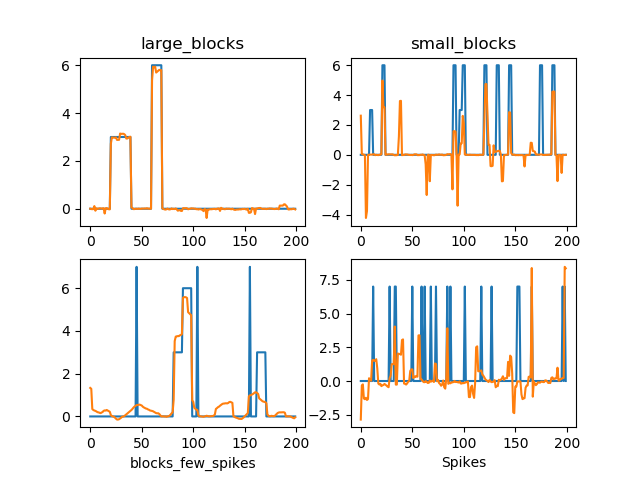
\includegraphics[width=0.7\textwidth]{../../out/figures/plot_fused.png}
\caption{Fused Lasso estimator applied to the four settings.}
\end{figure}
\subsection{Monte Carlo Simulation}

We conducted a Monte-Carlo simulation on the large blocks setting described above, to investigate the distribution of some specific estimated coefficients. The design matrix and error term were sampled from a standard normal distribution.  In each iteration, we generated new error terms, while the design matrix remained fixed. In this setup, the block structure was estimated 1000 times where the penalty constants were chosen by the grid-cv method.  In particular, we were interested in the distribution of four different points in the block structure. Namely, betas which are inside a block denoted by 'Center of the block', inside a block but at the edge of it 'Edge of the block', coefficients with value zero but which are next to a block 'Neighbouring to the block' and coefficients which are not next to a block 'Zero'. 
We observe that for both coefficients inside the block it seems like the estimator is normally distributed with bias since the true coefficient is 3. This bias is due to the shrinkage effect of the lasso and fusion penalty. For zero coefficients the distribution seems to be non-normal. This could be due to the bias introduced by the fusion penalty.
%Possible structures of coefficients for the simulation:
%\begin{enumerate}
%	\item plateaus (of different size) already implemented
%	\item plateaus and one(ore more) peaks
%	\item sparsity, but without plateaus
%	\item situations in which the lasso or fused lasso may not be appropriate (imposing a wrong prior):
%	\begin{enumerate}
%		\item no ordering of the features
%		\item no sparsity
%	\end{enumerate}
%\end{enumerate}
\begin{table}
	\centering
	\scriptsize
	\begin{tabular}{llrlrlrlrl}
\toprule
       &        & \multicolumn{2}{l}{MSE} & \multicolumn{2}{l}{Sensitivity} & \multicolumn{2}{l}{Specificity} & \multicolumn{2}{l}{Blocks} \\
Setting & Method &         &           &              &         &              &         &         &         \\
\midrule
Large\_blocks & Lasso &  167.86 &  (120.68) &         0.20 &  (0.06) &         0.93 &  (0.02) &    0.06 &  (0.08) \\
       & Fused &   28.53 &   (37.51) &         0.98 &  (0.05) &         0.92 &  (0.08) &    0.47 &   (0.3) \\
       & Fusion &   51.09 &   (56.56) &         0.96 &  (0.09) &         0.36 &   (0.3) &    0.46 &  (0.31) \\
Blocks\_few\_spikes & Lasso &  157.90 &  (106.22) &         0.21 &  (0.06) &         0.92 &  (0.02) &    0.05 &  (0.06) \\
       & Fused &   12.01 &   (19.98) &         0.77 &  (0.13) &         0.77 &  (0.11) &    0.31 &  (0.27) \\
       & Fusion &  116.89 &   (67.88) &         0.87 &  (0.13) &         0.12 &  (0.14) &    0.41 &  (0.29) \\
Small\_blocks & Lasso &  152.86 &   (65.75) &         0.19 &  (0.06) &         0.93 &  (0.02) &    0.04 &  (0.04) \\
       & Fused &   88.83 &   (47.11) &         0.49 &   (0.1) &         0.88 &  (0.05) &    0.13 &   (0.1) \\
       & Fusion &  538.98 &  (142.15) &         0.32 &  (0.46) &         0.00 &  (0.07) &    0.15 &  (0.24) \\
Spikes & Fasso &  467.54 &  (130.04) &         0.20 &  (0.07) &         0.97 &  (0.02) &     -- &   (--) \\
       & Fused &  119.90 &   (59.46) &         0.40 &  (0.11) &         0.82 &  (0.04) &     -- &   (--) \\
       & Fusion &  850.75 &  (183.45) &         0.26 &  (0.44) &         0.06 &  (0.23) &     -- &   (--) \\
\bottomrule
\end{tabular}
	
	\caption{Results of the simulation study.}
\end{table}
\section{Real Data Application} \label{sec: real data}

To investigate the fused lasso estimator in a real data setting we replicate an application from medical science described in \citep{spatial}.
We analyze data from Comparative Genomic Hybridization (CGH), an increasingly popular method for the molecular analysis of cancer.\footnote{The data was taken from https://web.stanford.edu/~hastie/StatLearnSparsity/data.html (the website was visited on 9th December 2018).}  
CGH provides an overview of changes in DNA sequence copy numbers in a tumor sample relative to a healthy control sample. Changes can be in form of losses, deletions, gains and amplifications \citep{cghmain}. The idea is that in cancer cells mutations can cause these changes . Biological knowledge suggest that it is typically segments of a chromosome, that means a couple of neighbouring genes, that are replicated and not single genes. 
The aim of the analysis of the data is to detect these regions of gains and losses of copy numbers.\\ 
%he DNA sequence copy number is then given as a function of chromosomal location throughout the entire genome, the genetic material of an organism \citep{cghsecond}. 
In the CGH experiment DNA sequence copy numbers are measured for selected genes on the chromosome. Unfortunately the data are very noisy and render some kind of smoothing necessary before being analyzable.
The fused lasso signal approximator is an appropriate method for this type of smoothing.
As seen above the estimator is designed for cases with $ p = n$ and a meaningful ordering of the coefficients.
Our data consists of 990 observations, where each observation is the $\log_2$ ration between the copy numbers of a gene in the tumor cells and the copy number in the healthy cells.  \\
If we regress the copy number on the genes, we have $p=n$.
Also, we expect the underlying vector of true copy numbers $\beta$ to be piecewise constant over contiguous regions of a chromosome. 
The result $\hat{\beta}_j$ of the fused lasso estimation can be interpreted as the estimated DNA copy number for gene $j$. In this setup the penalty constant $s_1$ controls the overall amount of alteration of the  DNA copy number and $s_2$ the frequency of the changes.
Applying the fused lasso estimator with the penalty terms $s_1 = 160$ and $s_2 = 15$ replicates the findings of \citep{spatial}, our result is visualized in figure \ref{cghdata}. The estimator suggests a main region, where DNA sequence copy number gains have possibly taken place and also wide regions of losses. Note that the fused lasso detects the region of gains although it is narrow.
\begin{figure}
	\centering
	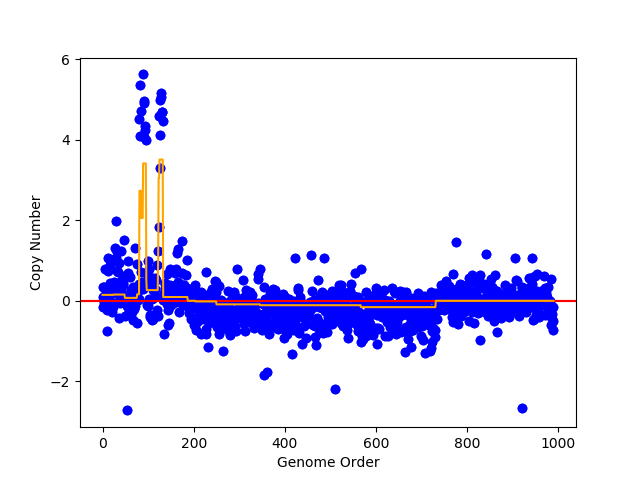
\includegraphics[width=0.6\textwidth]{../../out/figures/cgh_plot_beta.png}
	\caption{CGH Data}
	\label{cghdata}
\end{figure}
\FloatBarrier
\section{Conclusion}

W have studied two specific penalized regressions for high-dimensional data. The lasso for sparse settings and the fused lasso for sparse block settings. We showed that the fused lasso outperforms lasso in cases for which fused lasso was designed.
The choice of appropriate penalty constants is challenging and can be seen as a weakness of the fused lasso.
Our approach to the problem is cross-validation on a two dimensional grid. Due to complexity of the fused lasso minimization problem only few asymptotic results are available. However the results for the fused lasso signal approximator provide ideas for the general case. Our work could be extended to the two-dimensional fused lasso and to other model generalizations. 
%\begin{enumerate}
%	\item Neighbors generalize to neighboring areas  (for example image reconstruction for 2d case, cf. \citep{sparsity})
%	\item Several different choices for the penalties on neighboring coefficients (apart from the $\ell^1$-norm) are possible.
%	\item Assume a uniformly spaced index, can consider cases where the index variable has nonuniform values (see p.667 in \citep{sparsity})
%	\item Can consider case where the features are unordered.
%	\item generalizations on the penalties and on the model fit possible
%\end{enumerate}
 %\citep{adams1995hitchhiker}

\appendix
\addtocontents{toc}{\protect\setcounter{tocdepth}{1}}
\newpage

\section{Code}




%beispiel für manuelle eingabe
\lstset{title=Data generating function}
\begin{python}
def generate_data(n, p, num_simulations, number_blocks, length_blocks,
                  amplitude, spike_level, levels=False, spikes=0):
    """Generate the data for the simulation."""

    beta = np.zeros([p, num_simulations])
    for sim in range(num_simulations):
        beta[:, sim] = generate_beta(p, number_blocks, length_blocks,
                                       amplitude, levels, spikes, spike_level)
    mean = np.zeros(p)
    cov = np.identity(p)
    X = np.random.multivariate_normal(mean, cov, n)
    mean_eps = np.zeros(num_simulations)
    cov_eps = np.identity(num_simulations)
    epsilon = np.random.multivariate_normal(mean_eps, cov_eps, n)
    Y = np.matmul(X, beta) + epsilon

    return beta, X, epsilon, Y
\end{python}

\lstset{title=Generate $\beta$ with block strucure}
\begin{python}
def generate_beta(p, number_blocks, length_blocks, amplitude,
                  levels=False, spikes=0, spike_level):
    """Generate betas with desired block structure for
    simulation purposes."""

    container = np.zeros(p)
    max_blocks = math.floor(p / length_blocks)

    start_blocks = rd.sample(range(max_blocks), number_blocks)

    if levels:
        """
        If the blocks should not all have equal levels, 
        we will randomly chose
        the level of each block as either amplitude 
        or amplitude times 2.
        """
        amplitudes = [amplitude, amplitude*2]
        for block in start_blocks:
            amp = rd.choice(amplitudes)
            for i in range(p):
                if (i >= block * length_blocks) and (i < (block+1) *
                                                     length_blocks):
                    container[i] = amp

    else:
        for block in start_blocks:
            for i in range(p):
                if (i >= block * length_blocks) and (i < (block+1) *
                                                     length_blocks):
                    container[i] = amplitude

    if spikes != 0:
        non_blocks = []
        for i in range(p):
            if container[i] == 0:
                non_blocks.append(i)
        beta_spikes = rd.sample(non_blocks, spikes)
        for i in beta_spikes:
            container[i] = spike_level

    return container
\end{python}

\lstset{title=Functions which solve the optimization problem}
\begin{python}
import cvxpy as cp

def fused_lasso_dual(y, x, lambda1, lambda2):
    """Solve for given data and penalty constants the fused 
    lasso dual form."""
    
    p = len(x[1, :])
    b = cp.Variable(p)
    error = cp.sum_squares(x*b - y)
    obj = cp.Minimize(error + lambda1 * cp.norm(b, 1) +
                      lambda2 * cp.norm(b[1:p]-b[0:p-1], 1))
    prob = cp.Problem(obj)
    prob.solve()

    return b.value
    
def fused_lasso_primal(y,x,s1,s2):
    """Solve for given data and penalty constants the fused 
    lasso primal form."""
    
    p = len(x[1,:])
    b = cp.Variable(p)
    error = cp.sum_squares(x*b - y)
    obj = cp.Minimize(error)
    constraints = [cp.norm(b,1) <= s1, cp.norm(b[1:p]-b[0:p-1],1) <= s2]
    prob = cp.Problem(obj, constraints)
    prob.solve()

    return b.value
\end{python}

\lstset{title=flestimator.py}
\begin{python}
import cvxpy as cp
import numpy as np
from sklearn.base import BaseEstimator, RegressorMixin


class FusedLassoEstimator(BaseEstimator, RegressorMixin):
    """
    Fused Lasso Estimator that makes a penalized least squares regression
    where differences between neighbouring betas and non-zero betas get
    penalized.
    The optimization objective for Fused Lasso is:
        (1 / (2 * n_samples)) * ||y - Xb||^2_2
        s.t.        ||b||_1     <= s1
             sum(|b_i-b_{i-1]|) <= s2
    Technically this is a Convex optimization problem that is 
    solved by cvxpy.
    """
    def __init__(self, s1, s2):
        """ Called when initializing the Fused Lasso Estimator. """
        self.s1 = s1
        self.s2 = s2

    def fit(self, X, y=None):
        """
        The code for the fused lasso estimator. The penalties s1 and s2 are
        included as additional restriction equations.
        Examples
        --------
        >>> reg = FusedLassoEstimator( s1 = 1, s2 = 10).fit(X, y)
        """
        p = len(X[1, :])
        b = cp.Variable(p)
        error = cp.sum_squares(X*b - y)
        obj = cp.Minimize(error)
        constraints = [cp.norm(b, 1) <= self.s1, cp.norm(b[1:p]-b[0:p-1], 1)
                       <= self.s2]
        prob = cp.Problem(obj, constraints)
        prob.solve()
        self.beta = b.value

        return b.value

    def predict(self, X, beta=None):
        """This function returns the fitted y values."""

        return np.matmul(X, self.beta)
\end{python}

\lstset{title=Estimation}
\begin{python}
if __name__ == "__main__":
    reg_name = sys.argv[1]
    sim_name = sys.argv[2]
    sim_dict = json.load(open(ppj("IN_MODEL_SPECS", sim_name + ".json"),
                         encoding="utf-8"))
    with open(ppj("OUT_ANALYSIS", "data_{}_{}.pickle".
                  format(reg_name, sim_name)), "rb") as in12_file:
        beta_X_epsilon_Y = pickle.load(in12_file)

    """Data import from pickle files."""
    true_beta = beta_X_epsilon_Y[0]                  
    X = beta_X_epsilon_Y[1]                         
    epsilon = beta_X_epsilon_Y[2]                    
    y = beta_X_epsilon_Y[3]                          

    """Pull Information out of json file."""
    p = sim_dict["p"]
    n = sim_dict["n"]
    s1_min = sim_dict["s1_min"]
    s1_max = sim_dict["s1_max"]
    s2_min = sim_dict["s2_min"]
    s2_max = sim_dict["s2_max"]
    number_blocks = sim_dict['number_of_blocks']
    length_blocks = sim_dict['length_blocks']
    amplitude = sim_dict['amplitude']
    spike_level = sim_dict['spike_level']
    levels = sim_dict['levels']
    spikes = sim_dict['spikes']
    num_simulations = sim_dict['num_simulations']

    """Building containers to store simulation results."""
    beta_hat = np.empty((p, num_simulations))
    y_hat = np.empty((n, num_simulations))
    residuals = np.empty((n, num_simulations))

    """Calculation of optimal lambda."""
    lasso_grid = {
      's1': list(np.linspace(s1_min, s1_max, 20))
    }
    fused_grid = {
      's2': list(np.linspace(s2_min, s2_max, 20))
    }
    two_d_grid = [{
            's1': list(np.linspace(s1_min, s1_max, 20)),
            's2': list(np.linspace(s2_min, s2_max, 20))
        }]

    if reg_name == 'lasso':
        lasso_grid = {
            's1': list(np.linspace(1, 100, 50))
        }
        fused_grid = {
            's2': list(np.linspace(1000, 1200, 1))
        }

        two_d_grid = [{
            's1': list(np.linspace(1, 100, 50)),
            's2': list(np.linspace(1000, 1200, 5))
        }]

    if reg_name == 'fusion':
        lasso_grid = {
            's1': list(np.linspace(1000, 120, 1))
        }
        fused_grid = {
            's2': list(np.linspace(1, 50, 50))
        }
        two_d_grid = [{
            's1': list(np.linspace(1000, 1200, 5)),
            's2': list(np.linspace(1, 100, 50))
        }]

    clf = GridSearchCV(fle(lasso_grid, fused_grid), two_d_grid,
                       scoring='neg_mean_squared_error',
                       n_jobs=-1, iid=False, refit=True,
                       cv=None, verbose=0, pre_dispatch='2*n_jobs',
                       error_score='raise-deprecating',
                       return_train_score='warn')

    clf.fit(X, y[:, 1])
    penalty_cv = [clf.best_params_["s1"], clf.best_params_["s2"]]

    """Calculation of beta corresponding to optimal lambda."""
    for i in range(num_simulations):
        beta_hat[:, i] = fle(penalty_cv[0], penalty_cv[1]).fit(X, y[:, i])
        y_hat[:, i] = np.matmul(X, beta_hat[:, i])
        residuals[:, i] = y[:, i] - y_hat[:, i]

    container = [beta_hat, true_beta, penalty_cv, y_hat, residuals]
    with open(ppj("OUT_ANALYSIS", "simulation_{}_{}.pickle"
                  .format(reg_name, sim_name)), "wb") as out_file:
        pickle.dump(container, out_file)
\end{python}
\newpage

\lstset{title=Analysis}
\begin{python}
import pickle
import json
import numpy as np
import sys
import matplotlib.pyplot as plt
from bld.project_paths import project_paths_join as ppj


if __name__ == "__main__":
	""" waf """
	sim_name = sys.argv[2]
	reg_name = sys.argv[1]
	sim_dict = json.load(open(ppj("IN_MODEL_SPECS", sim_name + ".json"), 
	           encoding="utf-8"))
	with open(ppj("OUT_ANALYSIS", "simulation_{}_{}.pickle".
	format(reg_name, sim_name)), "rb") as in12_file:
		simulated_data = pickle.load(in12_file)



	# Load Data from pickle file
	beta_hat = simulated_data[0]
	true_beta = simulated_data[1]
	residuals = simulated_data[4]
	
	# Load parameters from .json files.
	p = sim_dict["p"]
	n = sim_dict["n"]
	s1_min = sim_dict["s1_min"]
	s1_max = sim_dict["s1_max"]
	s2_min = sim_dict["s2_min"]
	s2_max = sim_dict["s2_max"]
	number_blocks = sim_dict['number_of_blocks']
	length_blocks = sim_dict['length_blocks']
	amplitude = sim_dict['amplitude']
	spike_level = sim_dict['spike_level']
	levels = sim_dict['levels']
	spikes = sim_dict['spikes']
	num_simulations = sim_dict['num_simulations']
	
	
	container_analysis = []
	
	
	# Calculation of Mean Squared Error
	mse_list = []
	for i in range(num_simulations):
		mse_list.append(1 / n * np.sum(np.square(residuals[:,i]))
	
	container_analysis.append(np.mean(mse_list))
	container_analysis.append(np.std(mse_list))
	
	
	
	
	# number of relevant variables
	correct_nonzero = sum((beta_hat >= 0.30*amplitude)  & (true_beta > 0))
			      * 1 / np.sum(true_beta > 0,axis = 0)
	container_analysis.append(np.mean(correct_nonzero))
	container_analysis.append(np.std(correct_nonzero))
	
	
	
	#count number of correctly estimated zero coefficients
	percent_correct_zero = np.sum((np.absolute(beta_hat) <= 0.01) &
				      (true_beta == 0),
	axis=0) / np.sum(true_beta == 0,axis = 0)
	
	container_analysis.append(np.mean(percent_correct_zero))
	container_analysis.append(np.std(percent_correct_zero))
	
	
	#count the spikes
	spike_count = []
	if sim_dict["spikes"] >= 1:
		for i in range(num_simulations): 
	
			count = 0
	
			for j in range(p):
	
				if j == p-1:
					break
	
				if (j == 0) & (true_beta[1,i] == 0) 
				   	& 
				   	(beta_hat[j,i] > amplitude/2) 
					& (true_beta[0,i] > 0):
	
				count = count + 1
	
				if (j == (p-1)) & 
				  (beta_hat[(p-1), i] > 2) & (true_beta[p-2, i] == 0) 
				  & (true_beta[p-1, i] > 0):
				count = count + 1
				
				if (true_beta[j-1, i] == 0) 
				  & (true_beta[j+1, i] == 0) 
				  & (beta_hat[j, i] > amplitude/2) & (true_beta[j, i] > 0):
				
				count = count + 1
	
		spike_count.append(count)
		spike_count = np.array(spike_count) / spikes
		container_analysis.append(np.mean(spike_count))
		container_analysis.append(np.std(spike_count))
	
	else:
		container_analysis.append('--')
		container_analysis.append('--')

# To avoid dividing by zero in the spike setting since in that case the number of blocks is 0
if reg_name == 'spikes':
	number_blocks = 1


counter_blocks = np.sum(((beta_hat >= 0.50*amplitude) & (beta_hat <= 1.5*amplitude) 
& (true_beta == amplitude)) |
((beta_hat >= 0.75*levels) & (beta_hat <= 1.25*levels) 
& (true_beta == levels)),axis = 0)

percent_blocks = np.array(counter_blocks) / (length_blocks * number_blocks)
container_analysis.append(np.mean(percent_blocks))
container_analysis.append(np.std(percent_blocks))

with open(ppj("OUT_ANALYSIS", "analysis_{}_{}.pickle"
.format(reg_name, sim_name)), "wb") as out_file:
	pickle.dump(container_analysis, out_file)
\end{python}


%\lstset{title={tests}}
% \pythonexternal{rm_fused_lasso/src/model_code/fused_lasso_dual.py}

\section{Proofs}

\subsection{Convexity of solution set for fixed $\lambda$}
\begin{proof}
Define the objective function
\begin{align*}
h(\beta)=\|Y-X\beta\|_2^2+\lambda\|\beta\|
\end{align*}
Note that $h(\beta)$ is convex. Let $\beta_1$ and $\beta_2$ be two minimizers of $h(\beta)$ and let $\beta_3=\alpha\beta_1+(1-\alpha)\beta_2$ where $\alpha \in (0,1)$. Then due to convexity of $h(\beta)$ for any $\beta \in \mathbb{R}^p$ we have
\begin{align*}
h(\beta_3)&=h(\alpha\beta_1+(1-\alpha)\beta_2) \leq \alpha \underbrace{h(\beta_1)}_{\leq h(\beta)}+(1-\alpha)\underbrace{h(\beta_2)}_{\leq h(\beta)} \\ &\leq \alpha h(\beta)+(1-\alpha)h(\beta)=h(\beta) \\ &\Rightarrow \alpha\beta_1+(1-\alpha)\beta_2 \ \ \ \text{is also a minimizer.}
\end{align*}
Note that this implies that in case Lasso has two solutions there are uncountably many solutions.
\end{proof}

\subsection{Existence lasso and fused lasso} 
\begin{proof}
First of all note that for any $b$ with $||b||_1 > \frac{||Y||^2}{\lambda}$ the following inequality holds:
\begin{equation}
S_\lambda(b) \geq \lambda ||b||_1 > ||Y||^2 = S_\lambda(0),
\end{equation}
that means the Lasso criterion is smaller for $\tilde{b}=0$, so $b$ is not a solution.
Thus we have
\begin{equation*}
\hat{\beta}_\lambda^{l} = \argmin_{\beta \in\rm \mathbb{R}^p} S_\lambda(b) = \argmin_{\substack{\beta \in\rm \mathbb{R}^p\\ 
||b||_1 \leq \frac{||Y||^2}{\lambda}}} S_\lambda(b).
\end{equation*}
Observe that $A:=\{b\in \mathbb{R}^p: ||b||_1 \leq \frac{||Y||^2}{\lambda}\}$ is compact and the squared $\ell^2$ norm is a continuous function. By the extreme value theorem it follows that there always exists at least one solution to the minimization problem. \newline

\textbf{Existence Fused Lasso}
The proof for the existence of the fused lasso works similar as the one for the lasso. The set over which we minimize now needs to be a subset of the set $A$, so the set is also bounded. By the same argument as above no $b \in \mathbb{R}^p$ with $\sum_{j=2}^{p} |b_j - b_{j-1}| > \frac{||Y||^2}{\lambda_2}$ can be a solution to the minimization problem. The set $B := \{b:\sum_{j=2}^{p} |b_j - b_{j-1}| \leq \frac{||Y||^2}{\lambda_2} \}$ is also closed. Since the intersection of two closed sets is closed $A\cap B$ is closed and the intersection is bounded due to $A$ being bounded, thus it is compact. By the extreme value theorem a solution to the fused lasso problem exists.
\end{proof}

\subsection{Lemma \ref{sa: soft thresholding}}
\begin{proof} The basis of this proof can be found in \citep{friedman2007pathwise}.
%	We want  to show that the solution to this problem 
%	\begin{equation}
%	\frac{1}{2}  \sum_{i=1}^{6}(y_{i}-\beta_i)^2+\lambda_1\sum_{i=1}^p|\beta_i| + \lambda_2 \sum_{j=2}^6|\beta_j- \beta_{j-1} |
%	\end{equation} is equivalent to first calculate the solution for some lambda2  and $\lambda_1 =0$ and then soft thresholding it with $\lambda_1>0$. 
The idea of the proof is to show that the soft-thresholded estimator solves the gradient equations for the fused lasso problem with penalties $\lambda_1$ and $\lambda_2$. Since the gradient equations are necessary and sufficient for it to be a solution the proof is then complete. The subgradient equations for the fused lasso signal approximator for $\lambda_1,\lambda_2 > 0$ are given by:
	\begin{equation}
	-(y_j-b_j)+\lambda_1 r_j +\lambda_2 [t_j - t_{j+1}]=0, \footnote{The subgradient equation for $j = 1$ is slightly different (see \eqref{theo:subderivatives_fused}), but all of the arguments follow equivalently.}
	\end{equation}
	where $r_j$ and $t_j$ are as in theorem \eqref{theo:subderivatives_fused}.
	Assume we calculated a solution for $\lambda_1=0$ and $\lambda_2 > 0$ and denote it by $\hat{\beta}_0$. The soft thresholded version of it is given by $\hat{\beta}_{\lambda_1}=sgn(\hat{\beta}_0)(|\hat{\beta}_0|-\lambda_1)_{\text{+}}$.
	To this solution correspond specific values for $r_j$ and $t_j$. We denote them by $r_j(0)$ and $t_j(0)$. Since $\lambda_1=0$, we can chose $r_j(0)$ arbitrarily in $[-1,1]$ for all $j$ with $\hat{\beta}_{0,j}=0$ as the subgradient equations hold for all values. For later arguments set $r_j(0)=0$ for all $j$ with $\hat{\beta}_{0,j}=0$. For $j$ with $\hat{\beta}_{0,j} \neq 0$ soft-thresholding has not changed the sign $r_j$ of the coefficient. \\
	Observe that soft-thresholding also cannot change the ordering of coefficients of neighboring regressors. If one is larger than the other it will be at least as large as the other after soft-thresholding too. In case one of the new neighboring coefficients is unequal to zero thus $t_j(\lambda_1) = t_j(0)$. In case the two coefficients are equal after soft-thresholding we are free to chose $t_j(\lambda) \in [-1,1]$, we chose $t_j(\lambda)=t_j(0)$. So for all $\lambda_1 > 0$ and $j \in 2, \ldots, p$ we have $t_j(\lambda)=t_j(0)$ and we can simply denote it by $t_j$. \\
	We now plug the soft-thresholded estimator into the subgradient equations and derive values for $r(\lambda)$, such that the equations are equal to zero. When plugging in we need to distinguish two cases: \\
	
	\textbf{Case 1: ($|\hat{\beta}_{0,j}| > \lambda$)} In this case $\hat{\beta}_{\lambda,j} > 0$. Note that $\sgn(\beta)|\beta|=\beta$. Thus plugging the estimator into the subgradient equation and reordering of terms gives
	\begin{equation}
	g_j = -y_j+\hat{\beta}_{0,j} -\lambda_1 r_j(0) + \lambda_1r_j(\lambda_1)+ \lambda_2 [t_j - t_{j+1}].
	\end{equation} As $r_j(\lambda_1) = r_j(0)$ we obtain the subgradient equation of $\hat{\beta}_0$, which is zero as $\hat{\beta}_0$ is a solution.\\
	
	\textbf{Case 2: ($|\hat{\beta}_{0,j}|< \lambda_1$) } In this case $\hat{\beta}_{\lambda,j}=0$.
	The subgradient equation is given by
	
	\begin{equation}
		g_j = -y_j + \lambda_1 r_j(\lambda_1) + \lambda_2 [t_j -t_{j+1}].
	\end{equation}
Since we can chose $r_j(\lambda_1)$ to be anywhere between -1 and 1 we set it to $\frac{\hat{\beta}_{0,j}}{\lambda_1}$. This is an element of $[-1,1]$ as we are in the case $|\hat{\beta}_{0,j}|< \lambda_1$. The subgradient equation reduces to:
\begin{equation}
	-y_j + \hat{\beta}_{0} + \lambda_2[t_j - t_{j+1}].
\end{equation}
This is again zero as it is the subgradient equation of $\hat{\beta}_0$. \\
As $\lambda_1$ was chosen arbitrarily in the proof it holds for all $\lambda_1 > 0$.
\end{proof}

\newpage 

\section{Figures}

\subsubsection{Penalties}

\begin{figure}[h]
	\centering
	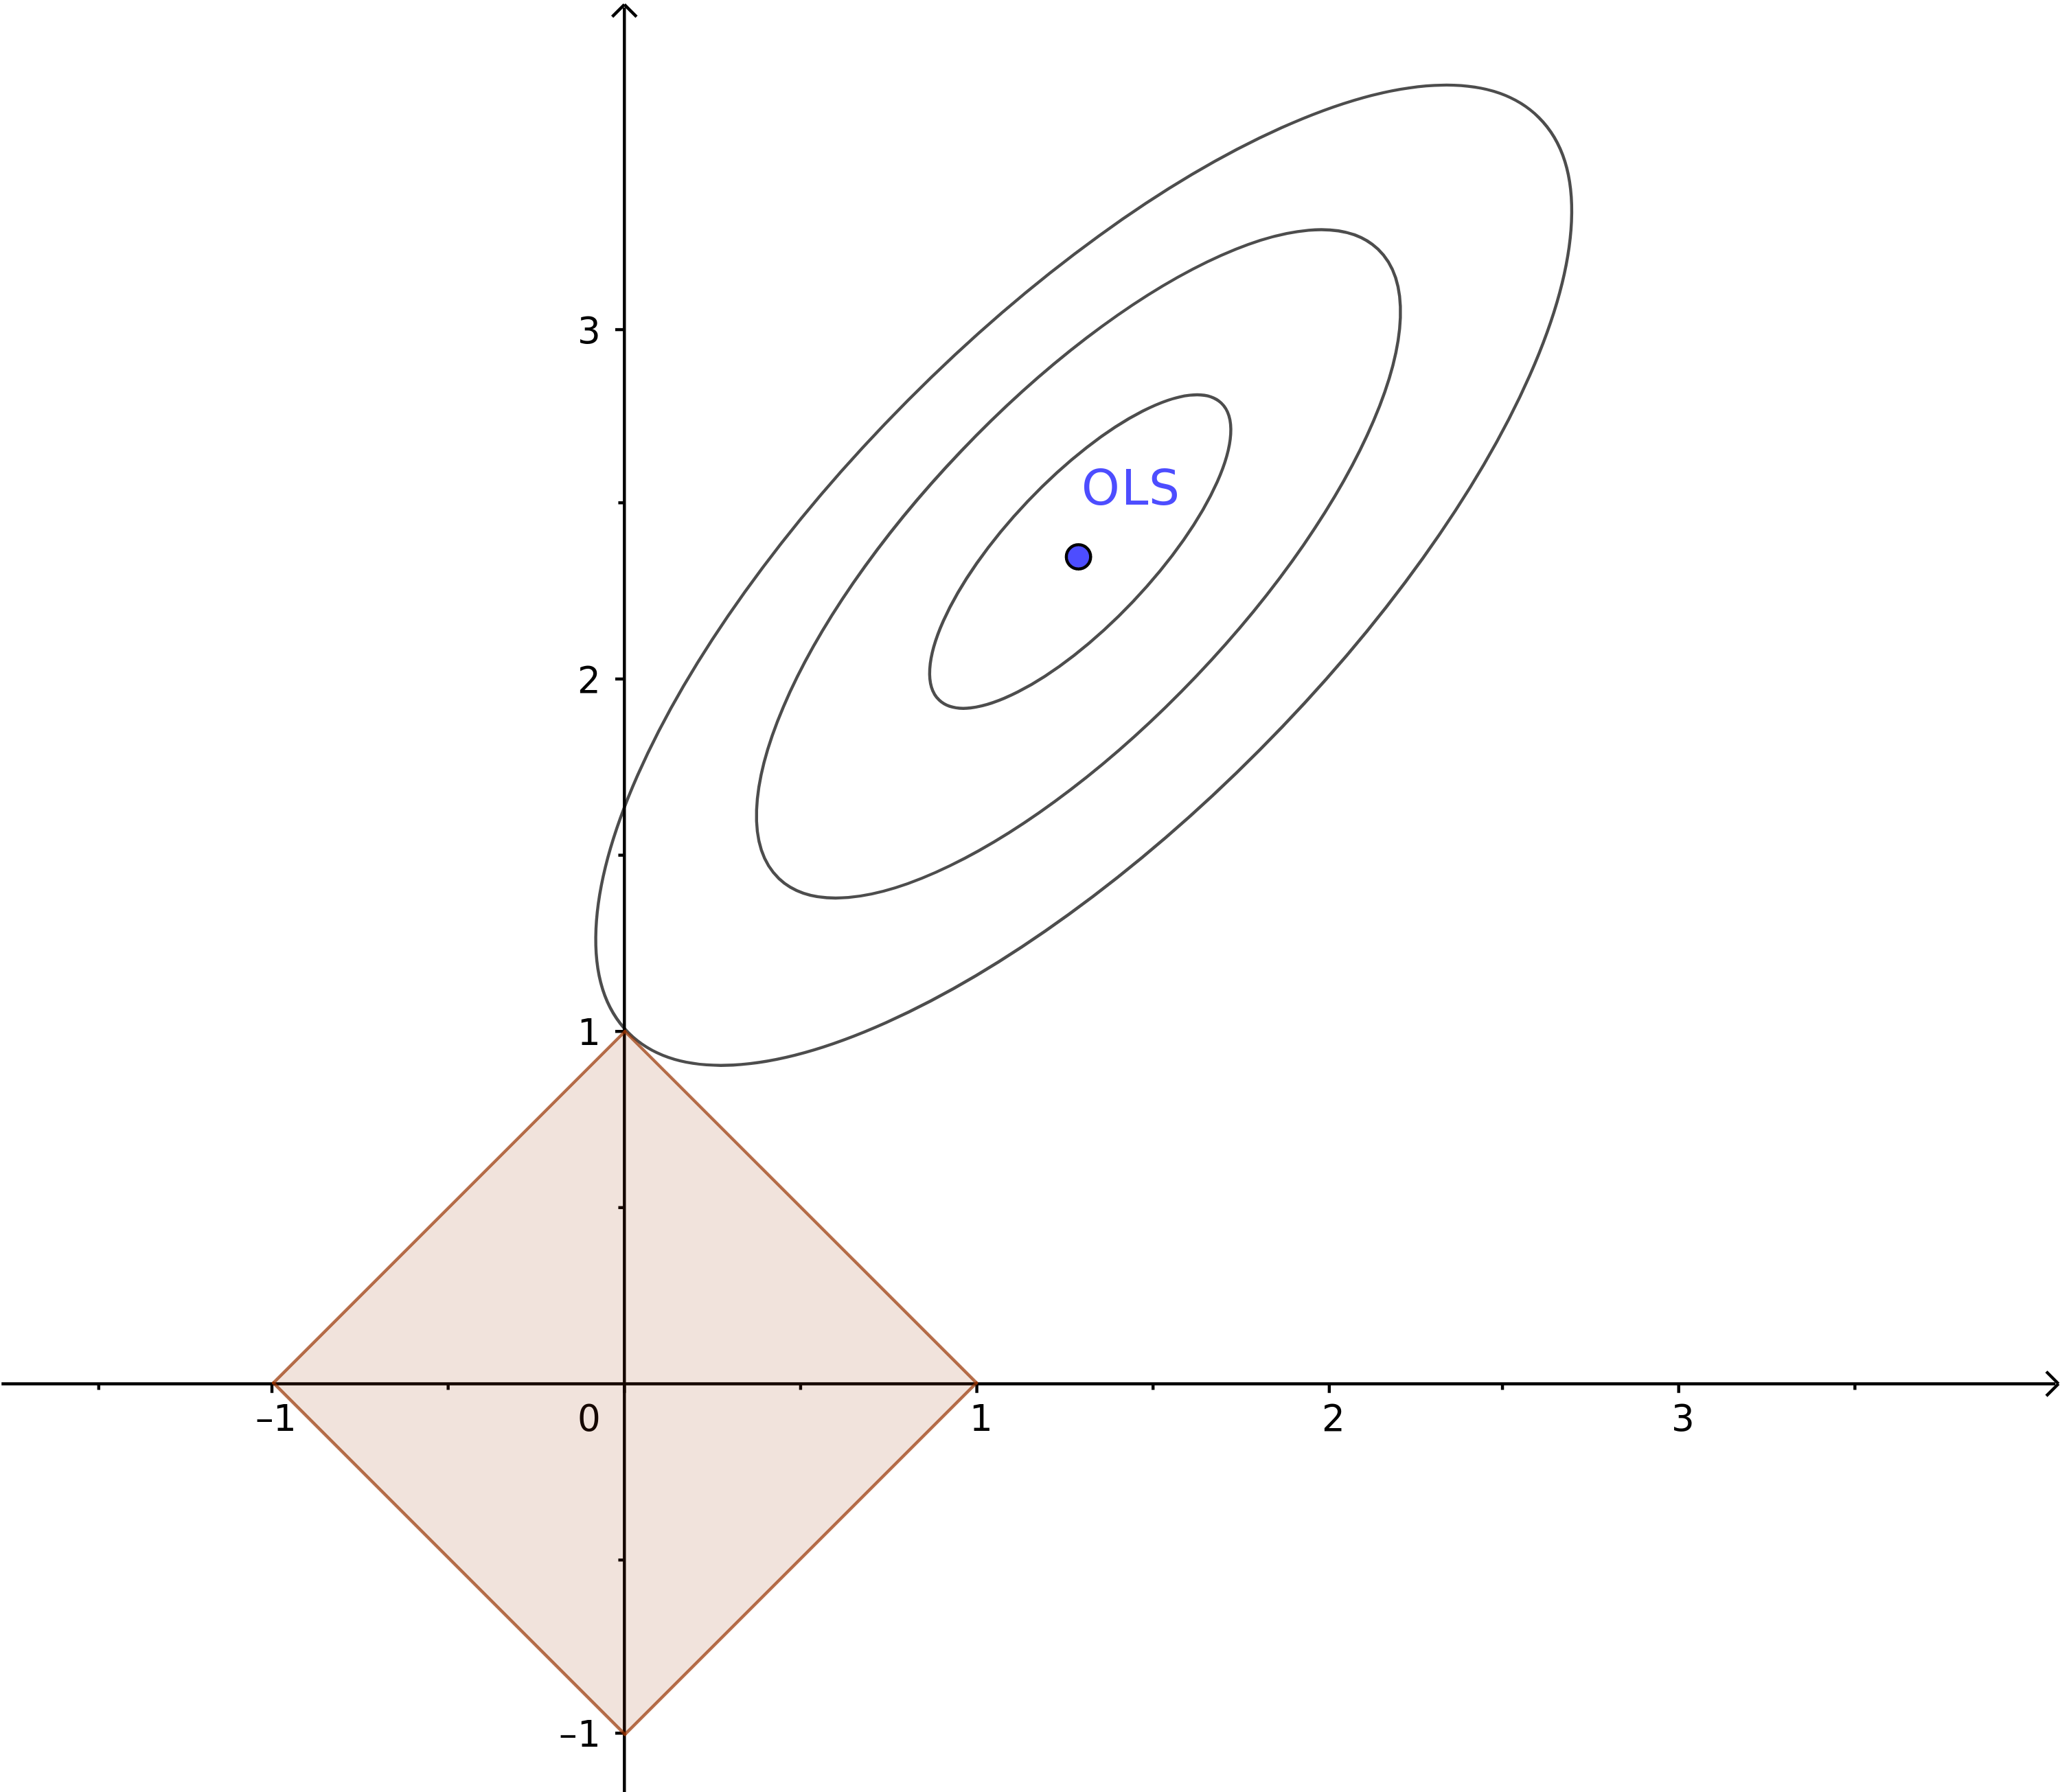
\includegraphics[width=0.7\textwidth]{external_figures/lasso_penalty}
	\caption{Lasso penalty and contour lines of least squares for $p=2$.}
	\label{lassopenalty}
\end{figure}

\begin{figure}[h]
	\centering
	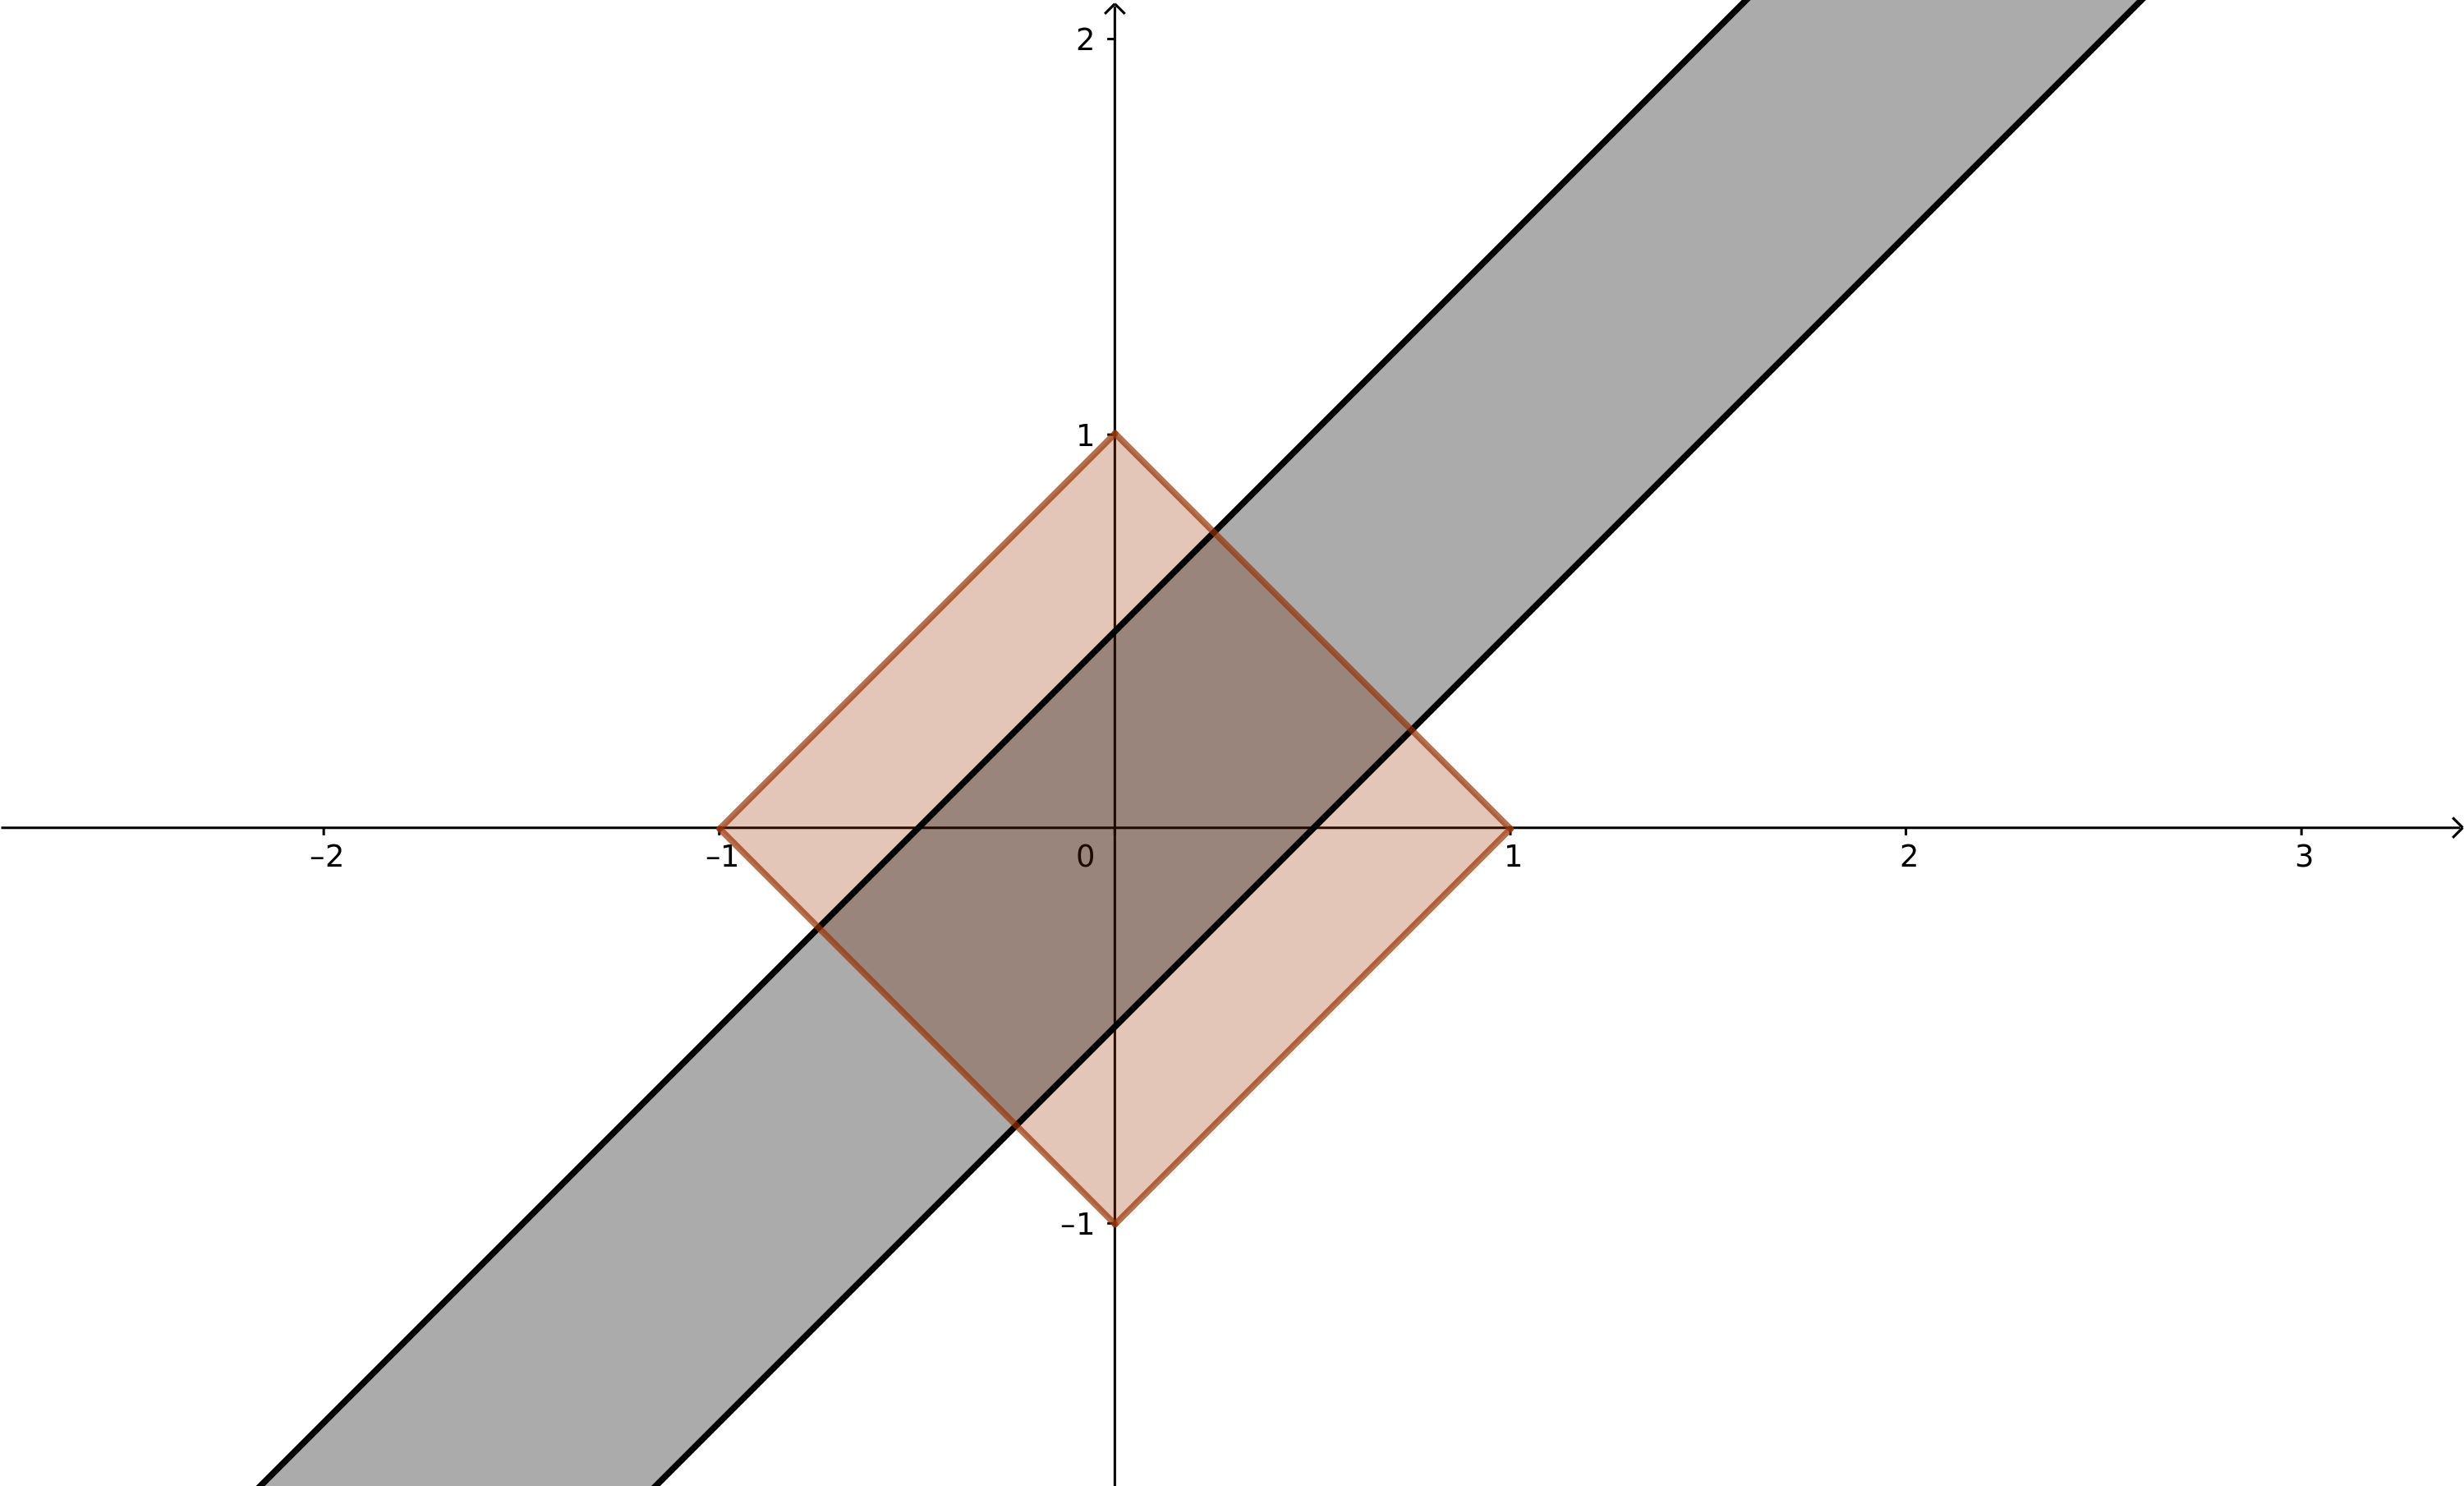
\includegraphics[width=0.5\textwidth]{external_figures/fused_and_lasso_penalty}
	\caption{Lasso penalty (red) and fused lasso penalty (gray)}
	\label{lassopenalty}
\end{figure}

\clearpage
\FloatBarrier
\subsubsection{Solution paths}
\begin{figure}
	\centering
	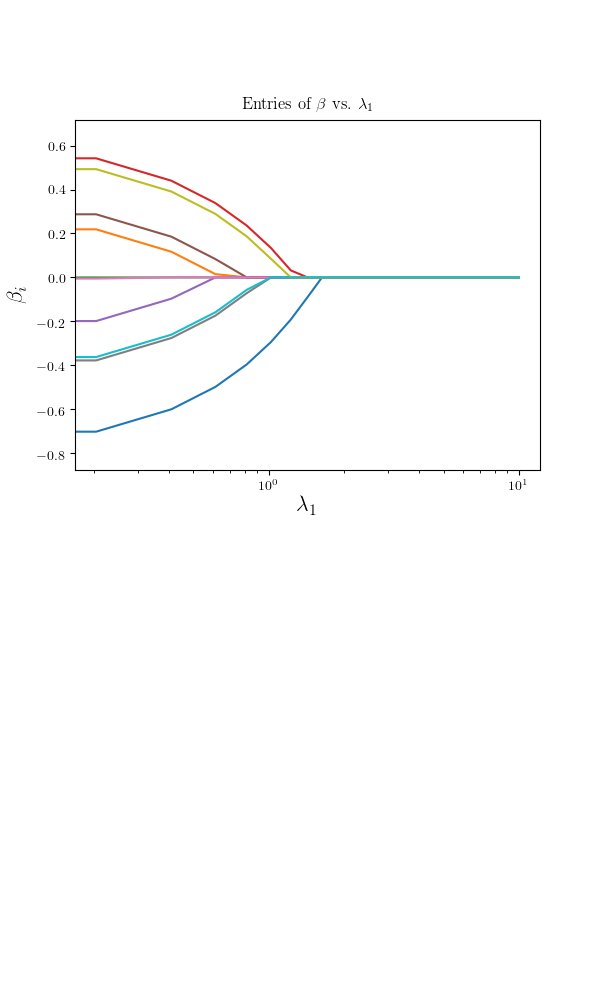
\includegraphics[width=.7\textwidth]{../../out/figures/plot_solutionpath_lasso.png}
	\caption{Solution path of the lasso}
	\label{fig:sollasso}
\end{figure}

\begin{figure}[h]
	\centering
	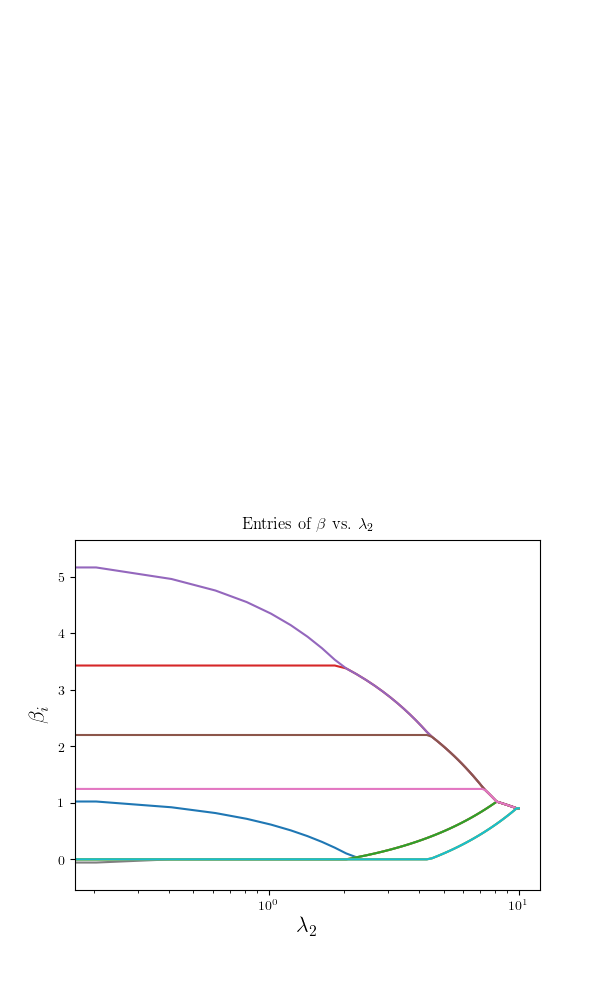
\includegraphics[width=0.7\textwidth]{../../out/figures/plot_solutionpath_fused_lasso.png}
	\caption{Solution path of the fused lasso for fixed $\lambda_1$ and $log(\lambda_2)$.}
	\label{lassopenalty}
\end{figure}
\clearpage
\FloatBarrier
\subsubsection{Heat maps}

\begin{figure}[h]
	\centering
	\begin{subfigure}[c]{0.45\textwidth}
		\includegraphics[width=1.1\textwidth]{../../out/figures/heatmap_blocks_few_spikes}
		\subcaption{Blocks with a few spikes}
	\end{subfigure}
	\begin{subfigure}[c]{.45\textwidth}
		\includegraphics[width=1.1\textwidth]{../../out/figures/heatmap_large_blocks}
		\subcaption{Large Blocks}
	\end{subfigure}
	\begin{subfigure}[c]{.45\textwidth}
		\includegraphics[width=1.1\textwidth]{../../out/figures/heatmap_small_blocks}
		\subcaption{Small blocks}
	\end{subfigure}
	\begin{subfigure}[c]{.45\textwidth}
		\includegraphics[width=1.1\textwidth]{../../out/figures/heatmap_spikes}
		\subcaption{Spikes}
	\end{subfigure}
	\caption{Blocks with a few spikes}
	\label{heatmap}
\end{figure}



\clearpage
\FloatBarrier
\subsubsection{Estimation}

	\begin{figure}[h]
		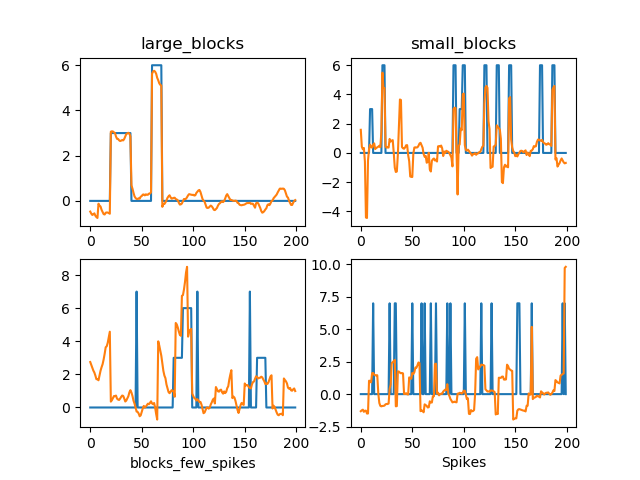
\includegraphics[width=\textwidth]{../../out/figures/plot_fusion.png}
		\caption{Fusion estimator applied to the four settings.}
	\end{figure}

\begin{figure}[h]
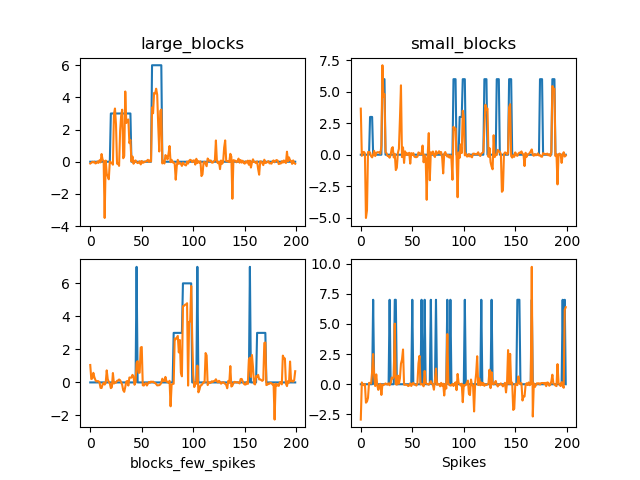
\includegraphics[width=\textwidth]{../../out/figures/plot_lasso.png}
\caption{Lasso estimator applied to the four settings.}	
\end{figure}

\begin{figure}[h]
	\includegraphics[width=\textwidth]{../../out/figures/monte_carlo_fused_large_blocks.png}
	\caption{Results of Monte-Carlo simulation..}	
\end{figure}


\clearpage

\bibliography{refs}

\end{document}

\begin{figure}[h]
	\centering
	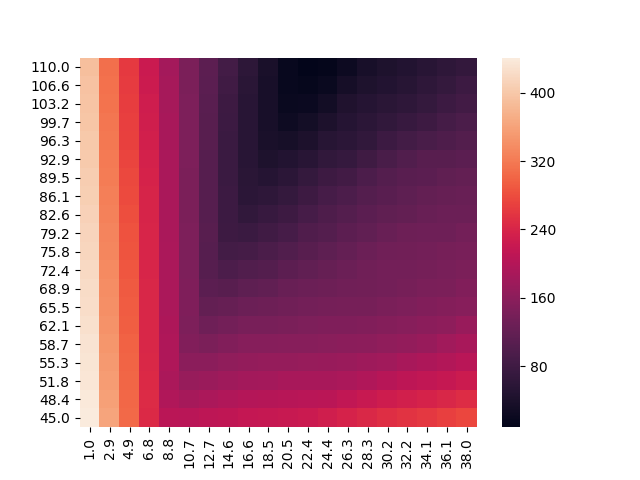
\includegraphics[width=0.6\textwidth]{../../src/sandbox/figures/heatmap_large_blocks_fused}
	\caption{Large Blocks}
\end{figure}

\begin{figure}[h]
	\centering
	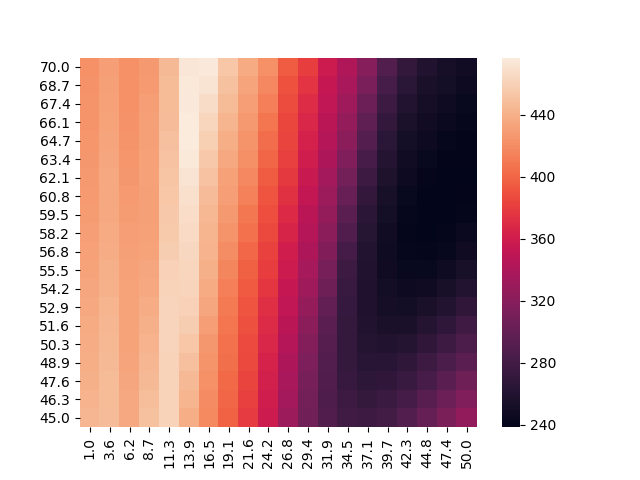
\includegraphics[width=0.6\textwidth]{../../src/sandbox/figures/heatmap_small_blocks_fused}
	\caption{Small blocks}
\end{figure}
\begin{figure}[h]
	\centering
	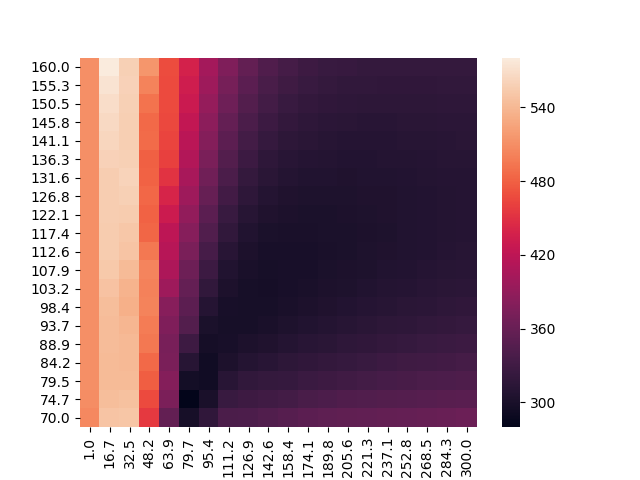
\includegraphics[width=0.6\textwidth]{../../src/sandbox/figures/heatmap_spikes_fused}
	\caption{Spikes}
\end{figure}
%
%\section{Lasso}
%    \subsection{Characterization of the LASSO-Solution}
%    For the Lasso criterion  
%    $$ \min_{b\in\RR^p}S_\lambda(b)=\frac{1}{n}(y_i-X_i^Tb)^2+\lambda||b||_1,\qquad \lambda>0$$
%    there exists $ b_\lambda\in\argmin_{b\in R^p}S_\lambda(b)$.\footnote{Proof: For }

